%% bare_conf.tex
%% V1.4b
%% 2015/08/26
%% by Michael Shell
%% See:
%% http://www.michaelshell.org/
%% for current contact information.
%%
%% This is a skeleton file demonstrating the use of IEEEtran.cls
%% (requires IEEEtran.cls version 1.8b or later) with an IEEE
%% conference paper.
%%
%% Support sites:
%% http://www.michaelshell.org/tex/ieeetran/
%% http://www.ctan.org/pkg/ieeetran
%% and
%% http://www.ieee.org/

%%*************************************************************************
%% Legal Notice:
%% This code is offered as-is without any warranty either expressed or
%% implied; without even the implied warranty of MERCHANTABILITY or
%% FITNESS FOR A PARTICULAR PURPOSE!
%% User assumes all risk.
%% In no event shall the IEEE or any contributor to this code be liable for
%% any damages or losses, including, but not limited to, incidental,
%% consequential, or any other damages, resulting from the use or misuse
%% of any information contained here.
%%
%% All comments are the opinions of their respective authors and are not
%% necessarily endorsed by the IEEE.
%%
%% This work is distributed under the LaTeX Project Public License (LPPL)
%% ( http://www.latex-project.org/ ) version 1.3, and may be freely used,
%% distributed and modified. A copy of the LPPL, version 1.3, is included
%% in the base LaTeX documentation of all distributions of LaTeX released
%% 2003/12/01 or later.
%% Retain all contribution notices and credits.
%% ** Modified files should be clearly indicated as such, including  **
%% ** renaming them and changing author support contact information. **
%%*************************************************************************


% *** Authors should verify (and, if needed, correct) their LaTeX system  ***
% *** with the testflow diagnostic prior to trusting their LaTeX platform ***
% *** with production work. The IEEE's font choices and paper sizes can   ***
% *** trigger bugs that do not appear when using other class files.       ***                          ***
% The testflow support page is at:
% http://www.michaelshell.org/tex/testflow/



\documentclass[conference]{IEEEtran}
% Some Computer Society conferences also require the compsoc mode option,
% but others use the standard conference format.
%
% If IEEEtran.cls has not been installed into the LaTeX system files,
% manually specify the path to it like:
% \documentclass[conference]{../sty/IEEEtran}

% Eigene packages
\usepackage[utf8]{inputenc} % für Umlaute im Dokument
\usepackage[ngerman]{babel} % für deutsche Silbentrennung
\usepackage[colorlinks=true]{hyperref} % für Hyperlinks / URLs
\usepackage{booktabs, tabularx, threeparttable} % für Tabellen
\usepackage{enumerate} % für die Nummerierung von Listen
\usepackage{amssymb}  % für \checkmark Häkchen-Zeichen
\usepackage[normalem]{ulem} % für Durchsteichen von Text \sout{Hello World}


% Eigene commands
\newcommand*{\TakeFourierOrnament}[1]{{%
\fontencoding{U}\fontfamily{futs}\selectfont\char#1}}
\newcommand*{\danger}{\TakeFourierOrnament{66}}

% Some very useful LaTeX packages include:
% (uncomment the ones you want to load)


% *** MISC UTILITY PACKAGES ***
%
%\usepackage{ifpdf}
% Heiko Oberdiek's ifpdf.sty is very useful if you need conditional
% compilation based on whether the output is pdf or dvi.
% usage:
% \ifpdf
%   % pdf code
% \else
%   % dvi code
% \fi
% The latest version of ifpdf.sty can be obtained from:
% http://www.ctan.org/pkg/ifpdf
% Also, note that IEEEtran.cls V1.7 and later provides a builtin
% \ifCLASSINFOpdf conditional that works the same way.
% When switching from latex to pdflatex and vice-versa, the compiler may
% have to be run twice to clear warning/error messages.






% *** CITATION PACKAGES ***
%
\usepackage{cite}
% cite.sty was written by Donald Arseneau
% V1.6 and later of IEEEtran pre-defines the format of the cite.sty package
% \cite{} output to follow that of the IEEE. Loading the cite package will
% result in citation numbers being automatically sorted and properly
% "compressed/ranged". e.g., [1], [9], [2], [7], [5], [6] without using
% cite.sty will become [1], [2], [5]--[7], [9] using cite.sty. cite.sty's
% \cite will automatically add leading space, if needed. Use cite.sty's
% noadjust option (cite.sty V3.8 and later) if you want to turn this off
% such as if a citation ever needs to be enclosed in parenthesis.
% cite.sty is already installed on most LaTeX systems. Be sure and use
% version 5.0 (2009-03-20) and later if using hyperref.sty.
% The latest version can be obtained at:
% http://www.ctan.org/pkg/cite
% The documentation is contained in the cite.sty file itself.






% *** GRAPHICS RELATED PACKAGES ***
%
\ifCLASSINFOpdf
  \usepackage[pdftex]{graphicx}
  % declare the path(s) where your graphic files are
  \graphicspath{{Bilder/}}
  % and their extensions so you won't have to specify these with
  % every instance of \includegraphics
  \DeclareGraphicsExtensions{.pdf,.jpeg,.png}
\else
  % or other class option (dvipsone, dvipdf, if not using dvips). graphicx
  % will default to the driver specified in the system graphics.cfg if no
  % driver is specified.
  % \usepackage[dvips]{graphicx}
  % declare the path(s) where your graphic files are
  % \graphicspath{{../eps/}}
  % and their extensions so you won't have to specify these with
  % every instance of \includegraphics
  % \DeclareGraphicsExtensions{.eps}
\fi
% graphicx was written by David Carlisle and Sebastian Rahtz. It is
% required if you want graphics, photos, etc. graphicx.sty is already
% installed on most LaTeX systems. The latest version and documentation
% can be obtained at:
% http://www.ctan.org/pkg/graphicx
% Another good source of documentation is "Using Imported Graphics in
% LaTeX2e" by Keith Reckdahl which can be found at:
% http://www.ctan.org/pkg/epslatex
%
% latex, and pdflatex in dvi mode, support graphics in encapsulated
% postscript (.eps) format. pdflatex in pdf mode supports graphics
% in .pdf, .jpeg, .png and .mps (metapost) formats. Users should ensure
% that all non-photo figures use a vector format (.eps, .pdf, .mps) and
% not a bitmapped formats (.jpeg, .png). The IEEE frowns on bitmapped formats
% which can result in "jaggedy"/blurry rendering of lines and letters as
% well as large increases in file sizes.
%
% You can find documentation about the pdfTeX application at:
% http://www.tug.org/applications/pdftex





% *** MATH PACKAGES ***
%
%\usepackage{amsmath}
% A popular package from the American Mathematical Society that provides
% many useful and powerful commands for dealing with mathematics.
%
% Note that the amsmath package sets \interdisplaylinepenalty to 10000
% thus preventing page breaks from occurring within multiline equations. Use:
%\interdisplaylinepenalty=2500
% after loading amsmath to restore such page breaks as IEEEtran.cls normally
% does. amsmath.sty is already installed on most LaTeX systems. The latest
% version and documentation can be obtained at:
% http://www.ctan.org/pkg/amsmath





% *** SPECIALIZED LIST PACKAGES ***
%
%\usepackage{algorithmic}
% algorithmic.sty was written by Peter Williams and Rogerio Brito.
% This package provides an algorithmic environment fo describing algorithms.
% You can use the algorithmic environment in-text or within a figure
% environment to provide for a floating algorithm. Do NOT use the algorithm
% floating environment provided by algorithm.sty (by the same authors) or
% algorithm2e.sty (by Christophe Fiorio) as the IEEE does not use dedicated
% algorithm float types and packages that provide these will not provide
% correct IEEE style captions. The latest version and documentation of
% algorithmic.sty can be obtained at:
% http://www.ctan.org/pkg/algorithms
% Also of interest may be the (relatively newer and more customizable)
% algorithmicx.sty package by Szasz Janos:
% http://www.ctan.org/pkg/algorithmicx




% *** ALIGNMENT PACKAGES ***
%
%\usepackage{array}
% Frank Mittelbach's and David Carlisle's array.sty patches and improves
% the standard LaTeX2e array and tabular environments to provide better
% appearance and additional user controls. As the default LaTeX2e table
% generation code is lacking to the point of almost being broken with
% respect to the quality of the end results, all users are strongly
% advised to use an enhanced (at the very least that provided by array.sty)
% set of table tools. array.sty is already installed on most systems. The
% latest version and documentation can be obtained at:
% http://www.ctan.org/pkg/array


% IEEEtran contains the IEEEeqnarray family of commands that can be used to
% generate multiline equations as well as matrices, tables, etc., of high
% quality.




% *** SUBFIGURE PACKAGES ***
%\ifCLASSOPTIONcompsoc
%  \usepackage[caption=false,font=normalsize,labelfont=sf,textfont=sf]{subfig}
%\else
%  \usepackage[caption=false,font=footnotesize]{subfig}
%\fi
% subfig.sty, written by Steven Douglas Cochran, is the modern replacement
% for subfigure.sty, the latter of which is no longer maintained and is
% incompatible with some LaTeX packages including fixltx2e. However,
% subfig.sty requires and automatically loads Axel Sommerfeldt's caption.sty
% which will override IEEEtran.cls' handling of captions and this will result
% in non-IEEE style figure/table captions. To prevent this problem, be sure
% and invoke subfig.sty's "caption=false" package option (available since
% subfig.sty version 1.3, 2005/06/28) as this is will preserve IEEEtran.cls
% handling of captions.
% Note that the Computer Society format requires a larger sans serif font
% than the serif footnote size font used in traditional IEEE formatting
% and thus the need to invoke different subfig.sty package options depending
% on whether compsoc mode has been enabled.
%
% The latest version and documentation of subfig.sty can be obtained at:
% http://www.ctan.org/pkg/subfig




% *** FLOAT PACKAGES ***
%
%\usepackage{fixltx2e}
% fixltx2e, the successor to the earlier fix2col.sty, was written by
% Frank Mittelbach and David Carlisle. This package corrects a few problems
% in the LaTeX2e kernel, the most notable of which is that in current
% LaTeX2e releases, the ordering of single and double column floats is not
% guaranteed to be preserved. Thus, an unpatched LaTeX2e can allow a
% single column figure to be placed prior to an earlier double column
% figure.
% Be aware that LaTeX2e kernels dated 2015 and later have fixltx2e.sty's
% corrections already built into the system in which case a warning will
% be issued if an attempt is made to load fixltx2e.sty as it is no longer
% needed.
% The latest version and documentation can be found at:
% http://www.ctan.org/pkg/fixltx2e


%\usepackage{stfloats}
% stfloats.sty was written by Sigitas Tolusis. This package gives LaTeX2e
% the ability to do double column floats at the bottom of the page as well
% as the top. (e.g., "\begin{figure*}[!b]" is not normally possible in
% LaTeX2e). It also provides a command:
%\fnbelowfloat
% to enable the placement of footnotes below bottom floats (the standard
% LaTeX2e kernel puts them above bottom floats). This is an invasive package
% which rewrites many portions of the LaTeX2e float routines. It may not work
% with other packages that modify the LaTeX2e float routines. The latest
% version and documentation can be obtained at:
% http://www.ctan.org/pkg/stfloats
% Do not use the stfloats baselinefloat ability as the IEEE does not allow
% \baselineskip to stretch. Authors submitting work to the IEEE should note
% that the IEEE rarely uses double column equations and that authors should try
% to avoid such use. Do not be tempted to use the cuted.sty or midfloat.sty
% packages (also by Sigitas Tolusis) as the IEEE does not format its papers in
% such ways.
% Do not attempt to use stfloats with fixltx2e as they are incompatible.
% Instead, use Morten Hogholm'a dblfloatfix which combines the features
% of both fixltx2e and stfloats:
%
% \usepackage{dblfloatfix}
% The latest version can be found at:
% http://www.ctan.org/pkg/dblfloatfix




% *** PDF, URL AND HYPERLINK PACKAGES ***
%
%\usepackage{url}
% url.sty was written by Donald Arseneau. It provides better support for
% handling and breaking URLs. url.sty is already installed on most LaTeX
% systems. The latest version and documentation can be obtained at:
% http://www.ctan.org/pkg/url
% Basically, \url{my_url_here}.




% *** Do not adjust lengths that control margins, column widths, etc. ***
% *** Do not use packages that alter fonts (such as pslatex).         ***
% There should be no need to do such things with IEEEtran.cls V1.6 and later.
% (Unless specifically asked to do so by the journal or conference you plan
% to submit to, of course. )


% correct bad hyphenation here
\hyphenation{op-tical net-works semi-conduc-tor}


\begin{document}
%
% paper title
% Titles are generally capitalized except for words such as a, an, and, as,
% at, but, by, for, in, nor, of, on, or, the, to and up, which are usually
% not capitalized unless they are the first or last word of the title.
% Linebreaks \\ can be used within to get better formatting as desired.
% Do not put math or special symbols in the title.
\title{Das Potenzial von Pair-Programming und testgetriebener Entwicklung für Berufseinsteiger}
% Sollten Berufseinsteiger in Paaren und testgetrieben Entwickeln?

% author names and affiliations
% use a multiple column layout for up to three different
% affiliations
\author{\IEEEauthorblockN{Christoph Hellmich}
\IEEEauthorblockA{Hochschule Bonn-Rhein-Sieg\\
Fachbereich Informatik\\
Sankt Augustin\\
Email: Christoph.Hellmich@smail.inf.h-brs.de}
\and
\IEEEauthorblockN{Mirella Espinoza}
\IEEEauthorblockA{Hochschule Bonn-Rhein-Sieg\\
Fachbereich Informatik\\
Sankt Augustin\\
Email: Mirella.Espinoza@smail.inf.h-brs.de}}
%\and
%\IEEEauthorblockN{James Kirk\\ and Montgomery Scott}
%\IEEEauthorblockA{Starfleet Academy\\
%San Francisco, California 96678--2391\\
%Telephone: (800) 555--1212\\
%Fax: (888) 555--1212}}

% conference papers do not typically use \thanks and this command
% is locked out in conference mode. If really needed, such as for
% the acknowledgment of grants, issue a \IEEEoverridecommandlockouts
% after \documentclass

% for over three affiliations, or if they all won't fit within the width
% of the page, use this alternative format:
%
%\author{\IEEEauthorblockN{Michael Shell\IEEEauthorrefmark{1},
%Homer Simpson\IEEEauthorrefmark{2},
%James Kirk\IEEEauthorrefmark{3},
%Montgomery Scott\IEEEauthorrefmark{3} and
%Eldon Tyrell\IEEEauthorrefmark{4}}
%\IEEEauthorblockA{\IEEEauthorrefmark{1}School of Electrical and Computer Engineering\\
%Georgia Institute of Technology,
%Atlanta, Georgia 30332--0250\\ Email: see http://www.michaelshell.org/contact.html}
%\IEEEauthorblockA{\IEEEauthorrefmark{2}Twentieth Century Fox, Springfield, USA\\
%Email: homer@thesimpsons.com}
%\IEEEauthorblockA{\IEEEauthorrefmark{3}Starfleet Academy, San Francisco, California 96678-2391\\
%Telephone: (800) 555--1212, Fax: (888) 555--1212}
%\IEEEauthorblockA{\IEEEauthorrefmark{4}Tyrell Inc., 123 Replicant Street, Los Angeles, California 90210--4321}}




% use for special paper notices
%\IEEEspecialpapernotice{(Invited Paper)}




% make the title area
\maketitle

% As a general rule, do not put math, special symbols or citations
% in the abstract
\begin{abstract}

\textit{Kontext und Motivation}: Für Hochschulabsolventen/innen eines Informatikstudiengangs ändert sich die Situation häufig grundlegend, sobald sie beginnen im industriellen Umfeld zu arbeiten. Die praktische Anwendung des theoretischen Wissens gewinnt im Beruf immer mehr an Bedeutung. Die Abschluss inhabende Person muss sich unter anderen mit Dingen, wie technischen Schulden, einer neuen Domäne oder der Arbeit in größeren Teams auseinandersetzten. Kommunikation und viel Feedback helfen Berufsunerfahrenen sich in dieser neuen Situation zurechtzufinden. Feedback und Kommunikation sind gleichzeitig auch zwei elementare Werte des Extreme Programmings (XP). Die Umsetzung dieser Werte erfolgt im XP unter anderen durch die beiden Praktiken Pair-Programming und testgetriebene Entwicklung.

% Abschluss inhabende Person; Person mit Abschluss
% Praktikum (direkt) nach Studienabschluss

%Das theoretische Wissen von Hochschulabsolventen ist oft ausgeprägter als ihre Fähigkeit das Wissen praktisch anzuwenden, da das Studium mehr auf die Theorie als auf die Praxis fokussiert ist. Für die Absolventen gewinnt die Anwendung des theoretischen Wissens häufig erst beim Berufseinstieg an Bedeutung. Zusätzlich unterscheidet sich die Situation in einem Unternehmen von der im Studium. Dies kann bei den Absolventen unter Umständen zu Unsicherheiten führen. Dem könnte das Vorgehen des Extrem Programmings entgegenwirken, dessen Werte u.a. Feedback, Kommunikation, Respekt und Courage sind.

\textit{Zentrale Fragen}: In der vorliegenden Arbeit wird untersucht, welche Potenziale Pair-Programming und testgetriebene Entwicklung, einzeln und in Kombination, für Berufseinsteiger haben.

%\textit{Ziele}: Anhand des aktuellen Stands der Wissenschaft soll eine Aussage über die Anwendung der beiden Praktiken gegeben werden.

%\textit{Wissenschaftlicher Beitrag}: Auswertung verschiedener Quellen in Hinblick auf das beschriebene Szenario. Ziehen eigener Rückschlüsse für die Beantwortung der gestellten Fragen. Beschreibung von Empfehlungen für die Lösung des Problems oder für weitere Untersuchungen. Dies gilt insbesondere bei der Betrachtung von der Kombination beider Prinzipien.

\textit{Ergebins}: Potenziale wurden vor allem in den Bereichen der Kommunikation, dem Übernehmen von Verantwortung, der Einarbeitung und der Stärkung des Selbstvertrauens identifiziert. Durch die Kombination von Pair-Programming und der testgetriebenen Entwicklung werden die meisten Herausforderungen angesprochen. Die Nutzung von nur einer der beiden Praktiken birgt ebenfalls viele Potenziale, kann in Einzelfall aber auch zu Problemen führen.

\end{abstract}


% no keywords



% For peer review papers, you can put extra information on the cover
% page as needed:
% \ifCLASSOPTIONpeerreview
% \begin{center} \bfseries EDICS Category: 3-BBND \end{center}
% \fi
%
% For peerreview papers, this IEEEtran command inserts a page break and
% creates the second title. It will be ignored for other modes.
\IEEEpeerreviewmaketitle

%!TEX root = bare_conf.tex

\section{Einleitung}

Oft haben Studierende während ihrer Ausbildung nur eingeschränkt Zeit praktische Erfahrungen in der Programmierung zu sammeln. Für Hausarbeiten, die nach Abschluss im Schrank/Papierkorb landen, ist die Codequalität bei der Entwicklung oft kein wichtiges Kriterium. Dies ändert sich bei dem Berufseinstieg, wenn Projekte über mehrere Jahre laufen und gepflegt werden müssen. Technische Schulden, schwer zu wartender oder ungetesteter Code können langfristig zum Scheitern eines Projekts führen. Dies sorgt unter Umständen dafür, dass sich Absolventen\footnote{Aus Gründen der besseren Lesbarkeit wird hier und im Folgenden auf die gleichzeitige Verwendung männlicher und weiblicher Sprachformen verzichtet. Sämtliche Personenbezeichnungen gelten gleichwohl für beiderlei Geschlecht.} an ihrem neuen Arbeitsplatz unter Druck gesetzt fühlen, selbst wenn sie die theoretischen Grundlagen beherrschen. Für den Arbeitgeber bedeutet die mangelnde Praxis der Absolventen, dass teure Fachkräfte bezahlt werden, die sich nicht nur in eine neue Domäne, sondern auch mit der praktischen Programmierung auseinandersetzten müssen, bevor sie für das Unternehmen wirtschaftlich einsetzbar sind. Feedback hilft Unsicherheiten bzw. Unklarheiten zu klären. Häufiges Feedback ist ein zentraler Wert von \textit{Extreme Programming} (XP). Erreicht wird dies im XP unter anderen durch die beiden Praktiken \textit{Pair-Programming} (PP) und \textit{testgetriebene Entwicklung} (TDD). Beim Pair-Programming wird die Software von zwei Entwicklern gemeinsam an einem Rechner implementiert. Die testgetriebene Entwicklung unterscheidet sich von der traditionellen Entwicklung (TLD) insofern, als dass die Tests nicht nach, sondern vor der Implementierung der Funktionalität geschrieben werden \cite{Beck2004ExtremeChange}.

In dem nachfolgenden Abschnitt \ref{sec:methodik} sind die Vorgehensweisen beschrieben, nach denen die Potenziale von der TDD und dem PP untersucht wurden. Im Anschluss sind im Abschnitt \ref{sec:Probleme} die Herausforderungen für Berufseinsteiger schematisch dargestellt. Darauf folgt im Abschnitt \ref{sec:tdd} und im Abschnitt \ref{sec:pp} die getrennte Untersuchung der Potenziale von TDD bzw. PP. Der nächste Abschnitt \ref{sec:TDD+PP} behandelt die Potenziale, wenn die Praktiken gemeinsam angewendet werden. Zum Schluss erfolgt in Abschnitt \ref{sec:ende} ein Fazit.

%!TEX root = bare_conf.tex

\section{Methodik} \label{sec:methodik}

\subsection{Literatur Review zur testgetriebene Entwicklung} \label{sec:tddMethode}
Für die Untersuchung der Potenziale der testgetriebenen Entwicklung für Programmieranfänger, wurde eine Literatur Review (LR) durchgeführt. In diesem Abschnitt wird das Vorgehen der LR beschrieben. Deren Auswertung steht in Abschnitt \ref{sec:tdd}.

\subsubsection{Suche} Für die Literatur Review wurden die digitalen Bibliotheken IEEE Explore, ACM Digital Library, SpringerLink und Science Direct - Elsevier durchsucht. Die Suchanfragen bezogen sich immer auf den Titel, der in der Bibliothek enthaltenden Dokumente. Als Suchbegriff wurden Variationen von „test-driven development“, „test-first“ und „tdd“ verwendet.

Alle Anfragen lieferten für die untersuchte Fragestellung relevante Ergebnisse. Nur die Suche nach Dokumenten die „tdd“ im Titel enthielten, listete vorrangig Dokumente ohne Bezug zur testgetriebenen Entwicklung auf. Daher wurde dieser Suche eine weitere Bedingung hinzugefügt, so dass nur Dokumente gesucht wurden, die „tdd“ im Titel \textit{und} das Wort „test“ im Abstrakt enthielten.

Die komplette Suche konnte für die Bibliothek IEEE Explorer in einer Suchabfrage zusammengefasst werden und ist nachfolgend repräsentativ für die Suche in den verschiedenen Bibliotheken dargestellt:\\
\\
\textsf{("Document Title":"test-driven development"{}\\
OR "Document Title":"test driven development"{}\\
OR "Document Title":"test-first"{}\\
OR "Document Title":"test first"{}\\
OR ("Document Title":"tdd"{} AND "{}Abstract":"test"))}.\\

Die Bibliotheken IEEE Explore, SpringerLink und Science Direct zeigten zu jedem Dokument Empfehlungen bzw. ähnliche Dokumente an. Diese Dokumente wurden ebenfalls mit ausgewertet. Insgesamt führte die Suche zu 38 Dokumente.

\subsubsection{Beschreibung der Ausschlusskriterien} Die gefundenen 38 Dokumente wurden jeweils hinsichtlich drei Kriterien untersucht. Die Kriterien können wie folgt zusammengefasst werden:
\begin{enumerate}[i]
\item Empirisch Studie mit Fokus auf TDD vs. TLD
\item Teilnehmer haben theoretische Kenntnisse aber wenig praktische Erfahrung in der Software-Entwicklung
\item Durchführung der Studie in der Industrie
\end{enumerate}
Nachfolgend sind die Kriterien beschrieben.

Erstens sollte es sich bei dem Dokument, um eine empirische Studie handeln. Auswirkung durch die testgetriebene Entwicklung sollten beispielsweise durch Versuche, Umfragen oder Interviews belegt oder widerlegt worden sein. In der Untersuchung im Abschnitt \ref{sec:tdd} stehen die Potenziale der TDD im Vergleich zu denen der traditionellen Entwicklung im Fokus. Daher war es wichtig, dass die TDD oder das traditionelle Vorgehen, auch als test-last Development (TLD) bezeichnet, nicht mit anderen Praktiken kombiniert wurde. Falls zusätzlich, andere Praktiken, wie beispielsweise \textit{Behaviour-Driven Development}, in einer Studie untersucht wurden, sollten die Aussagen der Studie über die TDD und TLD unabhängig davon gültig sein.

Zweitens sollten die Programmierfähigkeiten der Studienteilnehmer berücksichtig worden sein. Für die vorliegende Arbeit war insbesondere die Gruppe von Entwicklern interessant, die bereits einen Studienabschluss im Bereich des Software-Engineerings haben, aber noch keine oder nur wenig praktische Erfahrung in der Industrie vorweisen können.

Für das dritte Kriterium war das Umfeld in dem die Studie durchgeführt wurde entscheidend. Entsprechend der Fragestellung der vorliegenden Arbeit, wurden Studien bevorzugt, deren Untersuchung in einem industriellen Umfeld durchgeführt wurden.

\subsubsection{Anwendung der Ausschlusskriterien} Nach der Anwendung des ersten Kriteriums wurden 13 Dokumente aussortiert.

Die übrigen 25 Studien boten wenig bis keine Informationen über die Programmierfähigkeiten und den TDD-Erfahrungen der Studienteilnehmer. Als Kompromiss für das zweite Kriterium, wurden Studien aussortiert, deren Teilnehmer aus „ungraduated Students“ oder aus professionellen Entwicklern bestanden. Dadurch wurden 22 Studien aussortiert. Übrig blieben fünf Studien, deren Teilnehmer ausschließlich aus „graduated Students“ bestanden. Aussagen über die Programmierfähigkeiten der Studenten konnten aus den Studien selten extrahiert werden.

Von den Studien deren Teilnehmer einen Hochschulabschluss haben, aber nicht in der Industrie tätig sind, wurde keine im industriellen Umfeld durchgeführt. Das dritte Kriterium wurde daher \textit{nicht} angewandt.

Die übrigen gebliebenen drei Studien sind in Tabelle \ref{table:TDDLiteraturReview} beschrieben.

\begin{table*}[tbh]
\renewcommand{\arraystretch}{1.3}
\caption{Ergebnisse der TDD Literatur Review}
\label{table:TDDLiteraturReview}
\centering
\begin{tabularx}{\textwidth}{@{}Xp{0.29\textwidth}p{0.24\textwidth}p{0.07\textwidth}p{0.28\textwidth}@{}}
  \toprule
  Studie                                & Beschreibung                                                                                                                                                                                                              & Teilnehmer                                                                                                                                                     & Umfeld     & Ergebnis                                                                                                                                                                         \\ \midrule
  \cite{Causevic2012TestExperiment}     & Studenten wurden in zwei Gruppen eingeteilt. Eine Gruppe entwickelte nach TDD, die andere nach TLD. Der Quellcode, die Testfälle und ein Fragebogen, den die Studenten nach der Entwicklung ausfüllten, wurden analysiert. & 22 Studenten mit einem Abschluss.                                                                                                                                    & akademisch & Im Durchschnitt war die Qualität der Tests beider Gruppen gleich. Die Testabdeckung beider Gruppen war nahezu identisch. Die Summe der gefundene Fehler im Code, war bei der test-first-Gruppe geringer. Die test-first-Gruppe war im Durchschnitt eine Stunde vor der Kontrollgruppe mit der Aufgabe fertig.                                                                                                                \\
  \cite{Fucci2016AnApproach}            & Studenten haben in TDD und TLD entwickelt.                                                                                                                                                                                & 21 Studenten mit einem Abschluss                                                                                                                               & akademisch & Kein signifikanter Unterschied zwischen TDD und TLD in Testaufwand, externe Codequalität und Produktivität                                                                       \\
  \cite{Madeyski2010TheExperiment}      & Studenten wurden in test-first und test-last Gruppen eingeteilt.                                                                                                                                                          & Studenten mit einem Abschluss.                                                                                                                                       & akademisch & Kein signifikanter Unterschied zwischen den beiden Gruppen hinsichtlich der Branch Coverage und Mutation Score Indicator.                                                        \\ \bottomrule
\end{tabularx}
\end{table*}

\subsubsection{Snowballing} \label{sec:TDDMethodeSnow}

Aufgrund der geringen Anzahl an übrig gebliebenen Studien, wurde ein Snowballing mit Literatur Reviews (LR) durchgeführt, die während der oben beschrieben Suche ebenfalls gefunden wurden. Eine erneute Suche mit geänderten Suchabfragen blieb aus, da nach Mäkinen und Münch \cite{Makinen2014EffectsStudies} selbst bei hunderten von Publikationen die TDD erwähnen, nur wenige verwertbare Ergebnisse liefern würden.

In Tabelle \ref{table:TDDSnowballing} sind die betrachteten LRs aufgelistet. Wurden in einer LR die Informationen über die Teilnehmer einer empirischen Studie extrahiert und angegeben, ob es sich bei ihnen ausschließlich um Studenten mit einen Abschluss handelt, befindet sich in der Spalte \textit{Teilnehmer als Graduated identifiziert} ein \checkmark. Die Spalte \textit{Auswertung pro Studie} ist mit einem Häkchen versehen, falls separat für jede in der LR analysierte empirische Studie eine Auswertung der Ergebnisse angegeben worden ist, und die LR nicht nur eine zusammenfassende Auswertungen über alle analysierten Studien enthält. Verweist eine LR auf eine andere LR in der Tabelle, ist dies in der letzten Spalte \textit{Referenzen} kenntlich gemacht worden.

Mit Ausnahme von Rafique et al. \cite{Rafique2013TheMeta-Analysis} haben alle untersuchten LRs Aussagen über die interne Codequalität, externe Codequalität und Produktivität getroffen. Rafique et al. \cite{Rafique2013TheMeta-Analysis} verzichtete auf die Auswertung der internen Codequalität, da es dafür noch keine allgemein akzeptierte Metrik gäbe.

\begin{table}[b!]
\renewcommand{\arraystretch}{1.3}
\caption{Übersicht von TDD Literatur Reviews}
\label{table:TDDSnowballing}
\centering
\begin{threeparttable}
\begin{tabularx}{\columnwidth}{@{}XXXl@{}}
\toprule
Studien & Studienteilnehmer als „graduate“ identifiziert & Auswertung pro Studie & Referenzen \\ \midrule
Munir \cite{Munir2014ConsideringReview} & \multicolumn{1}{c}{\checkmark} & \multicolumn{1}{c}{\checkmark} & \cite{Rafique2013TheMeta-Analysis,Kollanus2010Test-DrivenApproach,Shull2010WhatDevelopment,Sfetsos2010EmpiricalReview,Jeffries2007TheProgramming,Causevic2011FactorsReview} \\
Rafique \cite{Rafique2013TheMeta-Analysis} & \multicolumn{1}{c}{\checkmark} & \multicolumn{1}{c}{\checkmark} & \cite{Kollanus2010Test-DrivenApproach,Turhan2010HowDevelopment,Shull2010WhatDevelopment} \\
Bissi \cite{Bissi2016TheReview} & \multicolumn{1}{c}{-} & \multicolumn{1}{c}{\checkmark} & \cite{Munir2014ConsideringReview,Rafique2013TheMeta-Analysis,Sfetsos2010EmpiricalReview,Jeffries2007TheProgramming,Causevic2011FactorsReview} \\
Kollanus \cite{Kollanus2010Test-DrivenApproach}\tnote{*} & \multicolumn{1}{c}{-} & \multicolumn{1}{c}{\checkmark} & - \\
Jeffries \cite{Jeffries2007TheProgramming} & \multicolumn{1}{c}{-} & \multicolumn{1}{c}{\checkmark} & - \\
Causevic \cite{Causevic2011FactorsReview} & \multicolumn{1}{c}{-} & \multicolumn{1}{c}{\checkmark} & - \\
Sfetsos \cite{Sfetsos2010EmpiricalReview} & \multicolumn{1}{c}{-} & \multicolumn{1}{c}{\checkmark} & - \\
Mäkinen \cite{Makinen2014EffectsStudies} & \multicolumn{1}{c}{-} & \multicolumn{1}{c}{\checkmark} & \cite{Turhan2010HowDevelopment,Rafique2013TheMeta-Analysis, Jeffries2007TheProgramming} \\
Turhan \cite{Turhan2010HowDevelopment} & \multicolumn{1}{c}{-} & \multicolumn{1}{c}{-} & - \\
Shull \cite{Shull2010WhatDevelopment} & \multicolumn{1}{c}{-} & \multicolumn{1}{c}{-} & \cite{Turhan2010HowDevelopment} \\ \bottomrule
\end{tabularx}
\medskip
      \footnotesize\textbf{Legende:}\smallskip
      \begin{tablenotes}\footnotesize
      \item[*] In \cite{Kollanus2010Test-DrivenApproach} werden die gleichen Studien wie in \cite{Kollanus2011CriticalDevelopment} untersucht.
      \end{tablenotes}
\end{threeparttable}
\end{table}

In Munir et al. \cite{Munir2014ConsideringReview} wurden sechs, \cite{Madeyski2010TheExperiment,Madeyski2005PreliminaryQuality,Gupta2007AnDevelopment,Muller2002ExperimentProgramming,Flohr2006LessonsTeachings,Flohr2005AnProblems}, und in Rafique et al. \cite{Rafique2013TheMeta-Analysis} zwei, \cite{Muller2002ExperimentProgramming,Flohr2006LessonsTeachings}, Studien identifiziert, deren Teilnehmer ausschließlich aus Studenten bestanden, die einen Abschluss hatten. Zusätzlich wurde in Rafique et al. \cite{Rafique2013TheMeta-Analysis} eine Studie \cite{Gupta2007AnDevelopment} erwähnt, in der 20 von den 22 Studienteilnehmern einen Abschluss hatten. Die Studie wurde ebenfalls ausgewertet. Abzüglich Überschneidungen zwischen den LRs kamen so weitere sieben Studien zusammen. Von den sieben Studien wurden drei, \cite{Flohr2006LessonsTeachings,Flohr2005AnProblems,Muller2001CaseEnvironment}, aussortiert, da in ihren Untersuchungen TDD zusammen mit Pair-Programming oder einer anderen Praktik aus XP angewendet wurde. Insgesamt wurden durch das Snowballing vier weitere Studien ermittelt.

\subsubsection{Ergebnis} Die drei gefundenen empirischen Studien aus der Suche in den digitalen Bibliotheken und die vier aus den untersuchten LRs wurden verglichen. Nur eine empirische Studie wurde sowohl bei der Suche in den digitalen Bibliotheken als auch bei der Untersuchung der LRs gefunden. Abzüglich dieser Überschneidung, standen für die Auswertung in Abschnitt \ref{sec:tdd} sechs Studien zur Verfügung.% siehe Tabelle \ref{table:TDDAuswertungKomplett}.

\subsection{Methodik Pair-Programming}

\subsubsection{Evaluierungsprotokoll} Für das Pair-Programming wurde ein Protokoll zur systematischen Evaluierung entwickelt. In diesem Protokoll werden Forschungsfragen bzgl. der Suchstrategien, Einschluss- und Ausschlusskriterien, Qualitätsbewertung, Datenextraktion und Synthesemethoden gestellt \cite{Kitchenham2007GuidelinesEngineering,Higgins2008Cochrane}.

\subsubsection{Forschungsfragen} Die folgenden Fragen wurden im Rahmen dieser Arbeit gestellt und beantwortet:

\begin{itemize}
\item Was ist Pair-Programming (PP)?
\item Welche Merkmale charakterisieren diese Methode?
\item Was spricht für und gegen PP?
\item Wo wird PP angewendet und warum?
\item Welchen Einfluss hat die Zusammensetzung der Programmiererpaare?
\item Nach welchen Kriterien werden die Gruppen gebildet?
\item  Welche Vorteile hat PP für Berufseinsteiger?
\item Welche Herausforderungen stellt PP an Berufseinsteiger?
\end{itemize}

\subsubsection{Literaturquellen und Suchkriterien} Die Literaturquellen und Suchkriterien umfassten elektronische Datenbanken. Folgende elektronische Datenbanken wurden durchsucht:

\begin{itemize}
\item  IEEE Explore
\item ACM Digital Library
\item ResearchGate
\item Google Scholar
\end{itemize}

Folgende Suchbegriffe wurden verwendet:
\begin{itemize}
\item Paarprogrammierung
\item Pair Programming OR Pair-Programming
\item Advantages OR Benefits
\item Expert-novice OR Expert AND novice
\end{itemize}

\subsubsection{Datenextraktion} Es wurde mehr als 30 Paper gefunden und ausgewertet. Im ersten Schritt wurden die Papers gespeichert. Anschließend wurden die Studien nach ihrem Inhalt tabellarisch klassifiziert. Schließlich wurden hier jene Veröffentlichungen berücksichtigt, die relevante Informationen enthielten (Tabelle \ref{table:PPStudien}).

\begin{table*}[t]
\renewcommand{\arraystretch}{1.3}
\caption{Ausgewertete Studien Pair-Programming}
\label{table:PPStudien}
\centering
\begin{tabularx}{\textwidth}{@{}lllllX@{}}
\toprule


Studienkontext & Studientyp & Anzahl Studien & Anzahl Teilnehmer & Referenzen & Anmerkungen \\ \midrule
Industrie & Umfrage & 3 & 782 & \cite{Bevan2002GuidelinesClass,Williams2006ExaminingProgrammers,Williams2010PairProgramming}  & Vor-und Nachteile, Qualitätsverbesserung \\
Industrie & Fallstudie & 2 & k.A & \cite{Bevan2002GuidelinesClass}  & Reduktion der Fehler \\
Industrie & Experiment & 1 & k.A & \cite{Williams2010PairProgramming}  & Überprüfung der Codequalität \\
Industrie & Studie & 1 & 15 & \cite{Bevan2002GuidelinesClass} & Überprüfung der Codequalität \\
Industrie & Bericht & 1 & k.A & \cite{Williams2010PairProgramming} & Reduktion der Test und Korrekturarbeiten \\
Wissenschaft & Studie & 3 & 1408 & \cite{Bevan2002GuidelinesClass,Williams2010PairProgramming}  & Überprüfung der Kompatibilität der Paare \\
Wissenschaft & Experiment & 1 & 41 & \cite{Bevan2002GuidelinesClass}  & Messung der Qualität des Codes \\
Industrie & Studie & 1 & 15 & \cite{Williams2006ExaminingProgrammers,Nosek1998TheProgramming}  & Gute Arbeitsatmosphäre; mehr Zuversicht im Team bzgl. der Produktqualität \\
Wissenschaft & Studie & 1 & 41 & \cite{Williams2000StrengtheningPair-Programming, Alshehri2014RankingProgramming}  & Vergleich "Solos vs. Paare" \\
Wissenschaft & Studie & 1 & k.A & \cite{Cockburn2001TheProgramming}  & Designqualität, Fehlerreduktion \\
Wissenschaft & Studie & 1 & 40 & \cite{Lui2006PairExpertexpert,Alshehri2014RankingProgramming} & Messung der Produktivität Anfänger-Experten \\ \bottomrule
\end{tabularx}
\end{table*}

\subsection{Vorgehen Kombination beider Praktiken}

Im Abschnitt \ref{sec:TDD+PP} lag der Fokus auf eine Interpretation der Ergebnissen der beiden vorhergehenden Abschnitten, in denen die Potentiale des TDDs und des PPs untersucht wurden. Infolgedessen wurde keine LR durchgeführt. Stattdessen wurden Studien verwendet, die aus den vorherigen beiden LRs aussortiert wurden, weil in diesen Studien die TDD und das PP gemeinsam untersucht wurden.

%!TEX root = bare_conf.tex

\section{Herausforderungen für Berufseinsteiger} \label{sec:Probleme}

Für Absolventen, die ihr Informatik Studium beendet haben, stellen sich beim Berufseinstieg in dem Bereich der Software-Entwicklung einige Herausforderungen.

Das Umfeld ändert sich in der Regel. Der Berufseinsteiger muss das Unternehmen und die Mitarbeiter kennenlernen. Wahrscheinlich wird er sich in eine neue Domäne einarbeiten müssen, je nach dem im welchen Bereich das Unternehmen tätig ist. Anders als die Kommilitonen im Studium, werden die Mitarbeiter nicht mehr alle auf den selben Niveau wie er sein. Einige Mitarbeiter sind beispielsweise für die Datenbank zuständig, andere für das Frontend oder für den Austausch mit dem Kunden. Jeder Mitarbeiter verfügt über Expertenwissen auf seinem eigenen Gebiet.

Vielleicht nutzt das Unternehmen neuere, ältere oder ganz andere Technologien als die, die der Berufseinsteiger aus seinem Studium kennt. Sehr wahrscheinlich ist, dass er sich in mindestens einer Technologie neu oder vertiefend auseinandersetzten muss. Wenn es sich bei seinem neuen Arbeitsplatz nicht, um ein Startup-Unternehmen handelt, wird vermutlich auch die Entwicklung an Altsystemen in seinen Aufgabenreich fallen. Es ist nicht unwahrscheinlich, dass er sich mit viel fremden Code auseinandersetzten muss. Zusätzlich wird das Unternehmen in der Regel bestimmte Werkzeuge für die Entwicklung, Versionsverwaltung, Fehlerberichte und ähnliches bereitstellen, mit denen er sich eventuell erst vertraut machen muss.

Die Arbeitsweise unterscheidet sich in einigen Punkten von der im Studium. Die Projekte werden meist längere Laufzeiten haben, als dies bei den Haus- oder Seminararbeiten im Studium der Fall war. Daher ist beispielsweise während der Entwicklung, vermehrt auf die Vermeidung von technischen Schulden zu achten. Es könnte sein, dass der Absolvent seine Arbeit nicht mehr ganz so frei, wie im Studium, einteilen kann. Arbeiten müssen evtl. plötzlich für einen kritischen Bugfix unterbrochen werden. Nachdem der Fehler behoben ist, muss die vorherige Arbeit ohne lange Einarbeitung fortgesetzt werden können. Anders als im Studium, wo Kommilitonen und Professoren meistens erreichbar sind und schnell Rückmeldung geben, ist der Austausch im Beruf mit anderen Projektbeteiligten, wie Mitarbeitern oder Kunden vielleicht nicht mehr ohne weiteres möglich. Die Mitarbeiter arbeiten vielleicht an einem anderen Standort oder haben Urlaub, der Kunde ist nicht erreichbar.

Baytiyeh und Naja \cite{Baytiyeh2011ChallengesCareer} befragten 217 Ingenieure, darunter 78\% männlich und 22\% weiblich, aus den Bereichen Bauingenieurwesen (32\%), Maschinenbau (23\%), Elektrotechnik (27\%), Technische Informatik (10\%) und Wirtschaftsingenieurwesen (8\%) über Herausforderungen die sie im Übergang vom Studium in den Beruf sehen. Die Teilnehmer arbeiteten im Libanon (43\%), der Region um den Persischen Golf (33\%), Europa und Nordamerika (14\%) und Afrika (10\%). Die größten Herausforderungen fallen in die drei Bereiche Kommunikation, Verantwortung und Selbstvertrauen. Die drei Bereiche wurden aus den Antworten der Teilnehmer, wie folgt abgeleitet:
\begin{itemize}
\item Kommunikation
\begin{itemize}
  \item Zusammenarbeit mit Menschen aus einem anderen Bereich
  \item Umgang mit dem Vorgesetzten
\end{itemize}
\item Verantwortung
\begin{itemize}
  \item Verantwortung übernehmen
  \item Verantwortlich für Ergebnisse
  \item Arbeitsdruck
  \item Selbständig arbeiten
\end{itemize}
\item Selbstvertrauen
\begin{itemize}
  \item Angst Fehler zu machen
  \item Nicht genug zu Wissen
  \item Selbständig lernen
\end{itemize}
\end{itemize}
Die Liste wurde mit den oben beschriebenen Herausforderungen kombiniert und dient in den nachfolgenden Abschnitten als Schema, um die Potenziale von Pair-Programming und der testgetriebenen Entwicklung zu bewerten.
\begin{itemize}
\item Kommunikation
\begin{itemize}
  \item Zusammenarbeit mit Menschen aus einem anderen Bereich, kein Expertenwissen, unterschiedliches Niveau
  \item Kommunikation mit Kunden nur eingeschränkt möglich
  \item Kommunikation mit Mitarbeitern nur eingeschränkt möglich
\end{itemize}
\item Verantwortung
\begin{itemize}
  \item Verantwortung übernehmen, längere Projektlaufzeiten
  \item Verantwortlich für Ergebnisse, technische Schulden
  \item Arbeitsdruck, Unterbrechungen
  \item Selbständig arbeiten
\end{itemize}
\item Selbständig lernen, Einarbeitung
\begin{itemize}
  \item Neue Domäne
  \item Neue Technologie
  \item Altsysteme / fremder Code
  \item Neue Werkzeuge
\end{itemize}
\item Selbstvertrauen
\begin{itemize}
  \item Angst Fehler zu machen
  \item Nicht genug zu Wissen
\end{itemize}
\end{itemize}

%umfeld
%\item Neue (fremde) Domäne, in die sich der Entwickler einarbeiten muss
%\item Nicht mehr alle auf dem gleichen Niveau, stärke Unterscheidung zwischen den oder verschiedene Fähigkeiten (Frontendexperte, Datenbankexperte...)
%\item Neues Umfeld, Unternehmensphilosophie, Mitarbeiter

%technisch
%\item Nicht auf den neusten Stand der Technik oder auf einem für das Unternehmen „zu“ neuem Stand. Andere Technologien. Viele neue Technologien.
%\item Altsysteme / viel fremder Code
%\item Vorgaben bestimmter (unbekannter) Werkzeuge für Versionsverwaltung, Entwicklung, Continous Delivery...

%arbeitsweise
%\item Lange Projektlaufzeiten. Technische Schulden.
%\item Weniger Freiheiten bei der Zeiteinteilung. Arbeit unterbrechen für ein Bugfix an einem anderen Projekt.
%\item Größe Projektteams möglich, evtl. verteilt in verschiedenen Städten/Ländern, (tatsächlich) unterschiedliche Rollen
%\item Kundenkontakt. Kunde nicht immer erreichbar.

%persönlich
%\item Mehr Verantwortung. Verantwortlich für die Ergebnisse. Unter Druck arbeiten. Selbständig Arbeiten \cite{Baytiyeh2011ChallengesCareer}
%\item Angest Fehler zu machen. Nicht genug zu wissen. Selbstänidg zu lernen \cite{Baytiyeh2011ChallengesCareer}

%!TEX root = bare_conf.tex

\section{Testgetriebene Entwicklung} \label{sec:tdd}

Die testgetriebene Entwicklung (TDD) ist eine der zentralen Praktiken des XPs, kann aber auch unabhängig davon angewendet werden. Die Methode setzt auf kurze Iterationen, in denen sowohl die Software als auch die Software-Architektur schrittweise entsteht. Anders als der Name vermuten lässt, ist TDD keine Teststrategie \cite{Janzen2005Test-drivenDirection}.

Nichtsdestotrotz beginnt jede Iteration mit dem Schreiben eines Tests. Anschließend wird genauso viel Code geschrieben, wie der Test für eine erfolgreiche Prüfung benötigt. Sobald der Test mit einem positiven Ergebnis durchgelaufen ist, kann, falls nötig, die bestehende Codebasis einem \textit{Refactoring} unterzogen werden \cite{Janzen2005Test-drivenDirection}.

Während des Refactoring wird die interne Struktur von existierenden und funktionierenden Programmcodes verbessert. Ziel ist es, den Code verständlicher zu machen, ohne neue Funktionalität hinzuzufügen \cite{Link2005SoftwaretestsEntwicklung}.

Etwas formaler kann die testgetriebene Entwicklung anhand von zwei Regeln beschrieben werden \cite{Beck2003TestExample}:
\begin{itemize}
\item Es soll nur neuer Code geschrieben werden, wenn ein Test fehlschlägt.
\item Redundanzen sollen eliminiert werden.
\end{itemize}
Diese beiden Regeln geben die Reihenfolge der Arbeitsschritte bei der Entwicklung vor \cite{Beck2003TestExample}:
\begin{enumerate}
\item Schreibe einen Test der kompiliert, aber fehlschlägt (Red).
\item Schreibe gerade so viel Code, dass der Test läuft (Green).
\item Überarbeite den Code, so dass keine Redundanzen mehr enthalten sind (Refactor).
\end{enumerate}
Insgesamt kann der Ablauf von der TDD mit dem kurzen Mantra „Red/Green/Refactor“\footnote{Fehlgeschlagene Tests werden in der Praxis oft durch die Farbe Rot und erfolgreiche Tests durch die Farbe Grün signalisiert.} beschrieben werden \cite{Beck2003TestExample}. In Abbildung \ref{fig:TDDvsTLD} sind die Unterschiede von TDD und TLD in Form zweier Aktivitätsdiagramme dargestellt.

\begin{figure*}[tbh]
\centering
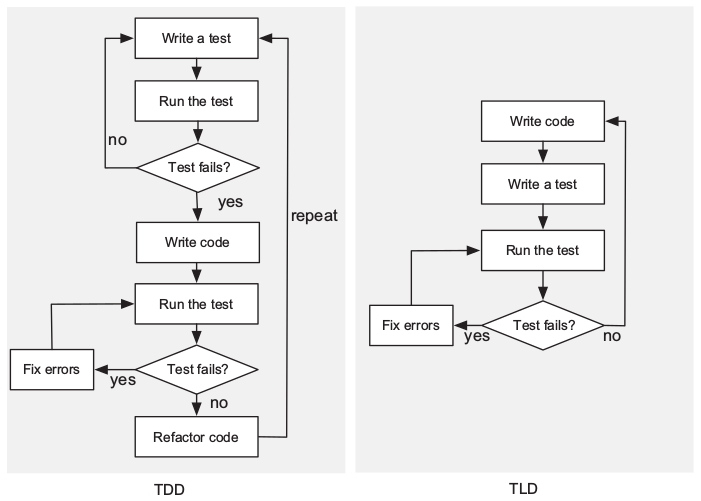
\includegraphics[scale=0.6]{tdd_vs_tld}
\caption{TDD vs. TLD, aus \cite{Munir2014ConsideringReview}}
\label{fig:TDDvsTLD}
\end{figure*}

Im Folgenden sind Vor- und Nachteile von der TDD aufgelistet, die häufig in der Literatur genannt werden. Im Anschluss sind positive und negative Auswirkung von der TDD beschrieben, die in Studien ermittelt wurden.

\subsection{Vorteile der testgetriebenen Entwicklung}  \label{sec:tddVorteile}
Nachfolgend sind Vorteile von der TDD beschrieben.

\subsubsection{Testabdeckung/Flexibilität} In der TDD soll neue Funktionalität nur dann hinzugefügt werden, wenn zuvor der entsprechende Test geschrieben wurde. Dadurch wird sichergestellt, dass nahezu der gesamte Code der Anwendung getestet ist. Die so erreichte hohe Testabdeckung, ermöglicht es, den gesamten Programmcode auf Fehler zu prüfen. Dies hilft dem Entwickler festzustellen, ob beispielsweise eine vorgenommene Änderung im Code, an einer anderen Stelle versehentlich einem Fehler in Programmablauf hervorruft. Der Code bleibt durch die hohe Testabdeckung flexibler.\cite{Martin2007ProfessionalismDevelopment, Janzen2005Test-drivenDirection}.

Die hohe Testabdeckung erlaubt es außerdem, eine Aussage über die Funktionsfähigkeit der Anwendung zu machen. Dies ist sowohl für die Planung als auch die Durchführung einer Softwareintegration wichtig \cite{Link2005SoftwaretestsEntwicklung}.

\subsubsection{Programmdesign} Eine Klasse lässt sich einfacher Testen, wenn sie keine oder wenig Abhängigkeit zu einer anderen Klasse besitzt. Durch die TDD werden die Entwickler ständig angehalten, auf eine lose Kopplung bei den Entwurf von Klassen zu achten \cite{Martin2007ProfessionalismDevelopment, Link2005SoftwaretestsEntwicklung,Yahya2015TheDevelopment}.

Allerdings heißt es auch in Martin \cite[S. 35]{Martin2007ProfessionalismDevelopment}: „Good designs aren’t free, and TDD doesn’t guarantee good designs. However, TDD provides powerful impetus to decouple, forcing developers to think through their designs in ways that they otherwise might not.“ Die TDD kann den Entwickler also nur dazu bringen auf das Design zu achten, aber dies muss nicht unweigerlich zu einen guten Design führen.

\subsubsection{Motivation} Bei der traditionellen Entwicklung, wird mit der Implementierung der Funktionalität begonnen und im Anschluss sollen die Tests geschrieben werden, um die Funktionalität zu prüfen. Häufig fehlt dem Entwickler jedoch die Motivation nach der Implementierung noch Tests zu schreiben. Er ist sich sicher, dass seine Implementierung fehlerfrei ist. Es ist für ihn dann oft interessanter, mit der Implementierung des nächsten Features zu beginnen. Die ohnehin geringe Motivation Tests zu schreiben, kann zusätzlich noch negativ beeinflusst werden, wenn die Abhängigkeiten zwischen den erstellten Klassen sehr groß sind, da dies das Schreiben von Tests erschwert. Beim TDD werden diese Probleme umgangen, da die Entwicklung mit dem Schreiben des Tests startet \cite{Link2005SoftwaretestsEntwicklung}.

In Shull \cite[S. 17]{Shull2010WhatDevelopment} heißt es, dass TDD hilft Schludrigkeiten zu verhindern und Disziplin beim Programmieren fördert: „He [Grigori] described working with a young, energetic programmer whose work unfortunately included many mistakes. Following TDD rigorously helped the programmer become more intentional in his work, thinking through the functionality he wanted to add. TDD doesn’t just require skill and discipline; it also helps develop them.“

\subsubsection{Dokumentation} Ein der Teil der Dokumentation des Codes erfolgt in Form von Tests. Die Tests geben Auskunft über die normale Verwendung von Klassen und deren Umgang mit Ausnahmen. Außerdem können die Tests als Kommunikationsgrundlage für den Austausch mit anderen Entwicklern dienen \cite{Link2005SoftwaretestsEntwicklung, Martin2007ProfessionalismDevelopment}.

Diese Dokumentation in Form von (Test-)Code wird von jedem Entwickler verstanden. Und dass die Tests bzw. die Dokumentation immer auf dem aktuellen Stand sind, ist durch das Vorgehen der TDD festgelegt. Jedoch muss für eine gute Lesbarkeit der Tests, bei deren Erstellung mit entsprechender Sorgfalt vorgegangen werden \cite{Martin2007ProfessionalismDevelopment}.

\subsubsection{Feedback/Unsicherheiten nehmen} TDD kann dabei helfen mit Unsicherheiten bei der Entwicklung umzugehen, die einen begegnet, wenn man auf ein schwer zu lösendes Problem trifft. Wenn Unsicherheiten einen zaghaft, weniger Kommunikativ und ängstlich gegenüber Fehlern machen, soll TDD den Entwickler, durch das kleinschrittige Vorgehen, unterstützen schnell zu lernen, klarer zu kommunizieren und konkretes Feedback zu finden \cite{Beck2003TestExample}.

Dies wird auf verschiedene Weise erreicht. Durch die vielen kurzen Iterationen erhält der Entwickler häufig Feedback. Eine fremde Schnittstelle kann mit der Hilfe von Tests schrittweise kennengelernt werden. Schwer zu lösende Probleme können in kleinere, einfacher zu lösende Probleme aufgeteilt und schrittweise bearbeitet werden. Dabei wird durch die Tests, für jeden Schritt ein Maß an Korrektheit sichergestellt, welches bei der Entwicklung ohne Tests fehlen würde. Durch die vielen Tests, erhält man ein sehr granulares Feedback, so dass weniger Zeit im Debugger verbracht werden muss, um die Ursache eines Fehlers zu finden  \cite{Beck2003TestExample, Link2005SoftwaretestsEntwicklung, Martin2007ProfessionalismDevelopment}.

\subsection{Nachteile der testgetriebenen Entwicklung} \label{sec:tddNachteile}
Kollanus \cite{Kollanus2011CriticalDevelopment} listet einige potentielle Probleme von TDD auf.

\subsubsection{Testabdeckung/Flexibilität} Typischerweise ist das Verhältnis zwischen Test- und Produktionscode eins zu eins. In großen Projekten kann eine große Menge von Testfällen zu verschiedenen Problemen führen. Zum einen kann die Entwicklungszeit durch die vielen Tests stark verzögert werden, wenn das Ausführen aller Tests beispielsweise mehrere Minuten in Anspruch nimmt. In solchen Fällen, kann nur noch eine Untermenge der Tests nach jeder Iteration durchlaufen werden. Zum anderen benötigt das Refactoring mehr Aufwand, wenn viele Testfällen von den Änderungen betroffen sind, und angepasst werden müssen \cite{Kollanus2011CriticalDevelopment}.

\subsubsection{Programmdesign} Das Fehlen einer vorab durchgeführten, detaillierten Designphase kann zu einem mangelhaften Design der Anwendung führen. Was wiederum ein umfangreiches Refacotring zur Folge haben kann \cite{Kollanus2011CriticalDevelopment}.

\subsubsection{Motivation} Es ist schwer die TDD im Unternehmen einzuführen, da es nicht leicht zu lernen ist und mehr Aufwand und Zeit benötig als zunächst von den Entwicklern erwartet wird. Außerdem ist die Grundeinstellung gegenüber TDD bei einigen negativ. Zum einen wird die Produktivität des Verfahrens hinterfragt. Zum anderen möchten einige Entwickler ungern ihre Art zu programmieren ändern. Und selbst, wenn die Entwickler von möglichen Vorteilen überzeugt sind, fehlt es an Motivation die TDD praktisch anzuwenden, da der Aufwand für den Einzelnen zu hoch ist \cite{Kollanus2011CriticalDevelopment}.

\subsubsection{Erforderliches Fähigkeitslevel} Obwohl der Ablauf der testgetriebenen Entwicklung überschaubar ist (Red/Green/Refactore), gibt es einige Probleme, auf die Anfänger zu Beginn schnell stoßen. Der Entwickler benötigt ein Big-Picture des Programms, um Tests schreiben zu können. Erfahrene Entwickler können das Design im Kopf entwerfen, und daher funktioniert die TDD für sie. Auf Anfänger trifft dies jedoch nicht zu. Neben dem Problem, zu bestimmen \textit{was} getestet werden soll, bereitet zusätzlich auch das \textit{wie} ein Tests geschrieben wird, einem Anfänger Probleme. Direkt beim Schreiben des ersten Tests, stellt sich beispielsweise die Frage, wie groß ein Test bzw. eine Iteration sein sollte. Insgesamt erfordert es viel Übung, bis ein Entwickler fähig ist, gute Testfälle zu schreiben. Anfänger können damit schnell überfordert sein \cite{Kollanus2011CriticalDevelopment, Beck2003TestExample}.

Die Umfrage von Aniche und Gerosa \cite{Aniche2010MostDevelopers} zeigt ebenfalls Schwierigkeiten, die die Entwickler mit der testgetriebenen Entwicklung haben. Sie befragten 218 Entwickler nach den Fehlern, die ihnen bei dem TDD-Prozess \textit{häufig oder immer} unterlaufen:
\begin{itemize}
  \item 26.61\% schreiben zu komplexe Testszenarien.
  \item 23.85\% führen ein Refactoring eines anderen Codeteils durch, anstatt den Teil zu korrigieren, der einen Tests fehlschlagen lässt.
  \item 19.72\% vergessen den Refactoring-Schritt durchzuführen.
  \item 15.14\% halten sich nicht an die Empfehlung, mit dem Schreiben des einfachsten Tests zu beginnen.
  \item 14.22\% vergessen zu prüfen, ob der gerade geschriebene Test tatsächlich fehlschlägt.
  \item 11.01\% verwenden schlechte Testname.
  \item 11,01\% implementieren nicht nur den nötigsten Code, damit der Test erfolgreich ist.
  \item 8.72\% vergessen den Testcode einem Refactoring zu unterziehen.
  \item 5.96\% vergessen am Ende einer Iteration alle Tests ausführen.
\end{itemize}

%Experten halten sich mehr an die Regeln des TDD als Anfänger. Die Zyklen/Arbeitsschritte sind kürzer ein die Länge einheitlicher als bei Anfängern. Dennoch konnten einige Anfänger schon nach einer Woche intensives Training ähnliche Werte erzielen, wie die Experten. Die Anzahl der Zyklen ist im Durchschnitt gleich, unter den Anfängern variiert diese Zahl jedoch stärker. Beide Gruppen haben gleich viele Änderungen an Codezeilen vorgenommen.Experte führen schneller Änderungen am Anwendungscode durch als die Anfänger. Die Anfänger sind bei der Änderung von Testcode schneller. Die Experten sind bei der Entwicklung signifikant schneller. Allerdings ist die Codeabdeckung der Experten-Testfälle größer. Größe der Programme ist unterschiedlich, aber nicht signifikant.
%Keine Hinweise, inwiefern die IDE unterstützung für TDD von den IDEs genutzt wurde \cite{Muller2007TheProcess}.

%\cite{Rafique2013TheMeta-Analysis} Entwicklererfahrung hat Einfluss auf TDD.

\subsubsection{Anwendbarkeit} Ungeachtet der Erfahrung des Entwicklers, kann es je nach Kontext sehr schwer sein, Tests zu schreiben. Dies gilt zum Beispiel für das Schreiben von Tests für Benutzeroberflächen. Ein weiteres Beispiel sind eingebettete Systeme, da es unter Umständen unmöglich sein kann, die Tests auf der Zielhardware auszuführen. In manchen Fällen ist die Anwendbarkeit der TDD abhängig von den zur Verfügungen stehenden Entwicklungswerkzeugen. Ohne die passenden Werkzeuge bzw. Werkzeugunterstützung, kann die TDD schnell zu Zeitaufwändig werden \cite{Kollanus2011CriticalDevelopment}.

\subsubsection{Positives Test-Bias} Bei der TDD werden vor allem positive Testfälle geschrieben, d.h. es wird getestet wie das System im Normalfall reagieren soll. Negative Testfälle, beispielsweise fehlerhafte Benutzereingaben, werden seltener überprüft. Jedoch werden durch negative Testfälle mehr defekte gefunden als durch positive Testfälle. Negative Testfälle sind daher für die Entwicklung wichtig, werden bei der TDD aber zu wenig beachtet \cite{Causevic2013EffectsExperiment}.

% Positive Test Bias: TDD ist keine Teststrategie

\subsection{Auswertung Studien} \label{sec:tddAuswertungStudien}

In diesem Abschnitt werden die Ergebnisse der gefundenen Studien aus Abschnitt \ref{sec:tddMethode} vorgestellt. Die Auswirkungen von der TDD werden in Experimenten, Befragungen, Fallstudien durch verschiedenen Metriken beschrieben. Munir et al. \cite{Munir2014ConsideringReview} listet acht Variablen auf, die in seinen untersuchten Studien häufig verwendet wurden: Produktivität, Aufwand/Zeit, Größe, externe Qualität, interne Codequaltät, Entwicklermeinung, Robustheit und  Konformität. Für jede Variable nennt er wiederum verschiedene Metriken. Nachfolgend werden die Ergebnisse zur Produktivität, externe Qualität und interne Codequalität näher betrachtet. Diese wurden von den meisten der betrachteten Studien verwendet.

\subsubsection{Produktivität} In der Studie \cite{Gupta2007AnDevelopment} von Gupta und Jalote wurden 22 Studenten gleichmäßig in zwei Gruppen eingeteilt. Eine Gruppe entwickelte testgetrieben, die andere traditionell. Die Gruppe die testgetrieben entwickelte, benötigte im Durchschnitt weniger Zeit zum Lösen von zwei vorgegebenen Programmieraufgabe. Der unterschied zwischen beiden Gruppen war jedoch nicht statistisch signifikant. Berechnet wurde die Produktivität mit der Formel \ref{eqn:TDDProduktivitaet}, wobei NCLOC für nicht auskommentierte Codezeilen steht und DE, die Zeit für die Entwicklung in Personenstunden beschreibt.

\begin{equation}
\label{eqn:TDDProduktivitaet}
Produktivitaet = \frac{NCLOC}{DE}
\end{equation}

Mülller und Hagner \cite{Muller2002ExperimentProgramming} teilte die 19 Teilnehmer seiner Studie ebenfalls in eine TDD-Gruppe und eine TLD-Gruppe ein, bestehend aus 10 bzw. 9 Studenten. Die Arbeit der Teilnehmer wurde in zwei Phasen eingeteilt. In der erste Phase wurde eine Anwendung implementiert. In der zweiten Phase führten die Studenten Akzeptanztest aus und behoben gegebenenfalls Fehler in ihrer Implementierung. Für die Evaluation der Produktivität wurden verschiedene Zeiten und Brüche verglichen. Dazu gehörte die Zeit, die für die die komplette Aufgabe benötigt wurde, die Zeit die für die Implementierungsphase benötigt wurde und das Verhältnis zwischen den beiden zuvor genannten Zeiten. Hinsichtlich der für die Aufgabe insgesamt benötigten Zeit, wurde kein Unterschied zwischen den beiden Gruppen festgestellt.

An der Studie von Causevic et al. \cite{Causevic2012TestExperiment} nahmen 14 Studenten teil. Sie wurden in zwei Gruppen eingeteilt. Die eine Gruppe nutzte die TDD, um eine vorgegebene Aufgabe zu lösen. Die andere Gruppe ging traditionell vor.  Die TDD-Gruppe war im Durchschnitt eine Stunde vor der TLD-Gruppe mit der Entwicklung fertig. Dies war jedoch nicht statistisch signifikant.

In der Studie von Fucci et al. \cite{Fucci2016AnApproach} entwickelten 21 Studenten einen Tag testgetrieben und einen Tag traditionell. Es wurden 40 Beobachtungen von 20 gültigen Teilnehmern analysiert. Dabei konnten keine Unterschiede hinsichtlich der Produktivität zwischen der TDD und der TLD festgestellt werden.

In zwei Studien neigten die Entwickler die testgetrieben entwickelten dazu, produktiver zu sein \cite{Gupta2007AnDevelopment,Causevic2012TestExperiment}. Drei Studien konnten keinen Unterschied in der Produktivität zwischen TDD und TLD feststellen \cite{Gupta2007AnDevelopment,Muller2002ExperimentProgramming,Fucci2016AnApproach}.  Werden jedoch nur die statistisch signifikanten Ergebnisse betrachtet, konnte weder die TDD noch die TLD als produktivere Praktik identifiziert werden.

\subsubsection{Externe Codequalität} An der Studie von Madeyski \cite{Madeyski2005PreliminaryQuality} nahmen 188 Studenten teil. Die Studenten wurden in vier Gruppen eingeteilt. Für diesen Abschnitt sind zwei Gruppen interessant. Die eine Gruppe entwickelte testgetrieben und bestand aus 34 Studenten. Die andere Gruppe entwickelte traditionell und bestand aus 32 Studenten. Der von der TDD-Gruppe geschriebene Code bestand weniger Akzeptanztests als der Code der TLD-Gruppe. Die externe Codequalität war statistisch signifikant geringer.

Auch in Gupta und Jalote  \cite{Gupta2007AnDevelopment} wurde die externe Codequalität durch die Anzahl erfolgreich durchlaufener Akzeptanztests ermittelt. Die Studienteilnehmer mussten zwei Programmieraufgaben lösen. Für die eine Programmieraufgabe war die externe Codequalität der TDD-Gruppe statistisch signifikant besser. Bei der anderen Aufgabe wurde kein statistisch signifikanter unterschied hinsichtlich der externe Codequalität zwischen den beiden Gruppen festgestellt. Für diese Aufgabe war die Anzahl der bestandenen Akzeptanztest bei der TLD-Gruppe höher, was eine bessere externe Codequalität vermuten lässt.

In Müller und Hagner \cite{Muller2002ExperimentProgramming} wurde die Anzahl der Fehler ebenfalls durch Akzeptanztest gemessen. Die externe Codequalität der TDD-Gruppe war nach der Implementierungsphase statistisch signifikant geringer. Nachdem die Studienteilnehmer Zeit hatten, die durch die Akzeptanztest aufgedeckten Fehler zu beheben, war die externe Codeqaulität der TDD-Gruppe ein wenig, jedoch nicht statistisch signifikant, besser als die der TLD-Gruppe.

Am Ende des Versuchs in Causevic et al. \cite{Causevic2012TestExperiment} wurde auf die Lösung jedes Teilnehmers, die Tests aller anderen Teilnehmer angewändet. Die fehlgeschlagenen Assertions dieser Tests wurden jeweils für jeden Teilnehmer gezählt und ausgewertet. Der Code der Teilnehmer die testgetrieben entwickelten, hatten im Durchschnitt weniger Defekte  als der Code der Teilnehmer die traditionell entwickelten. Der Unterschied war jedoch nicht statistisch signifikant.

Fucci et al. \cite{Fucci2016AnApproach} kam in seiner Sudie zu dem Ergebnisse, dass es kein Unterschied zwischen der TDD und der TLD hinsichtlich der externe Codequalität gibt. Die Codequalität wurde mit Hilfe von Akzeptanztests gemessen.

Für die externe Codequalität zeigt sich ein gemischtes Bild. In einer Studie gibt es keinen Unterschied zwischen TDD und TLD \cite{Fucci2016AnApproach}. Drei Studien erhalten keine statistisch signifikanten Ergebnisse. Davon tendieren in zwei der Studien die Teilnehmer, die TDD anwenden, zu besseren Ergebnissen \cite{Muller2002ExperimentProgramming, Causevic2012TestExperiment}. Die andere Studie kommt zu einem entgegengesetzten Resultat. In dieser liefert die TLD-Gruppe besseren Ergebnissen \cite{Gupta2007AnDevelopment}. Zwei Studien kommen zu statistisch signifikanten Ergebnissen. In \cite{Gupta2007AnDevelopment} schneidet TDD signifikant besser ab. Und in \cite{Madeyski2005PreliminaryQuality} ist wiederum TLD signifikant im Vorteil gegenüber TDD.

\subsubsection{Interne Codequalität} In der Studie von Madeyski \cite{Madeyski2010TheExperiment} wurden 19 Studenten in zwei Gruppen eingeteilt. Die TLD-Gruppe bestand aus zehn Studenten, die TDD-Gruppe aus neun. Zwischen den beiden Gruppen wurde kein statistisch signifikanter Unterschied hinsichtlich des Branch-Coverage gemessen. Die durchschnittliche Branch-Coverage  der TDD-Gruppe war, um 8\% Punkte höher.

Die Branch-Coverage wurde in Müller und Hagner \cite{Muller2002ExperimentProgramming} gemessen, nachdem die Aufgabe der Teilnehme vollständig abgeschlossen war. Die Ergebnisse der Messungen beider Gruppen waren ähnlich. Es konnte kein statistisch signifikanten Unterschied festgestellt werden.

In Causevic et al. \cite{Causevic2012TestExperiment} wurde die Code-Coverage der Teilnehmer untersucht. Im Durchschnitt war die Code-Covergage der TDL- und der TDD-Gruppe nahezu identisch.

Drei Studien haben die interne Codequalität untersucht. Zwei Studien konnten keinen Unterschied zwischen der TDD und der TLD feststellen \cite{Muller2002ExperimentProgramming,Causevic2012TestExperiment}. In \cite{Madeyski2010TheExperiment} war die Testabdeckung der Teilnehmer, die testgetrieben entwickelten, geringfügig höher.

\subsection{Potenziale für Berufseinsteiger} \label{sec:TDDPotenzial}

Die Auswertung der Studien nach den Metriken Produktivität, externe Codequalität und interne Codequalität in Abschnitt \ref{sec:tddAuswertungStudien} ist in Tabelle \ref{table:TDDAuswertungStudien} zusammengefasst. Die Auswertung hat gezeigt, dass viele Studien, einzeln und zusammengenommen, noch keine eindeutigen Ergebnisse liefern. Ob die TDD oder die TLD verwendet wird, scheint insgesamt keinen oder kaum Auswirkung auf die Produktivität, externe Codequalität und interne Codequalität zu haben. Nach Fucci et al. \cite{Fucci2016ATest-Last} besteht kein Unterschied zwischen der TDD und der TLD, und Vorteile ergeben sich allein durch das schrittweise Vorgehen.

\begin{table}[bth]
\renewcommand{\arraystretch}{1.3}
\caption{Auswertung TDD-Studien}
\label{table:TDDAuswertungStudien}
\centering
\begin{threeparttable}
\begin{tabularx}{\columnwidth}{@{}llll@{}}
\toprule
Studie & Produktivität & Externe Codequalität & Interne Codequalität \\ \midrule
\cite{Madeyski2010TheExperiment} & k.A. & k.A. & =\tnote{+} \\
\cite{Madeyski2005PreliminaryQuality} & k.A. & - & k.A. \\
\cite{Gupta2007AnDevelopment}\tnote{A1} & = & + & k.A. \\
\cite{Gupta2007AnDevelopment}\tnote{A2} & =\tnote{+} & =\tnote{-} & k.A. \\
\cite{Muller2002ExperimentProgramming} & = & =\tnote{+} & = \\
\cite{Causevic2012TestExperiment} & =\tnote{+} & =\tnote{+} & = \\
\cite{Fucci2016AnApproach} & = & = & k.A. \\ \bottomrule
\end{tabularx}
\medskip
      \footnotesize\textbf{Legende:}\smallskip
      \begin{tablenotes}\footnotesize
      \item = keine statistisch signifikanten Auswirkungen
      \item +/- statistisch signifikant positive/negative Auswirkungen von TDD gegenüber TLD
      \item[+/-] positive/negative Tendenzen von TDD gegenüber TLD
      \item[A1] Aufgabe 1
      \item[A2] Aufgabe 2
      \end{tablenotes}
\end{threeparttable}
\end{table}

Nachfolgend sind die Vor- und Nachteile der TDD aus dem Abschnitt \ref{sec:tddVorteile} zusammengefasst. Manche Punkte, wie z.B. die Testabdeckung, konnten sowohl als Vorteil als auch als Nachteil ausgelegt werden.
\begin{itemize}
\item Vorteile
\begin{enumerate}
  \item Testabdeckung/Flexibilität
  \item Programmdesign
  \item Motivation
  \item Dokumentation
  \item Feedback/Unsicherheiten nehmen
\end{enumerate}
\item Nachteile
\begin{enumerate}
  \item Testabdeckung/Flexibilität
  \item Programmdesign
  \item Motivation
  \item Erforderliches Fähigkeitslevel
  \item Anwendbarkeit
  \item Positives Test-Bias
\end{enumerate}
\end{itemize}

Die Auswertung in Abschnitt \ref{sec:tddAuswertungStudien} hat gezeigt, wie schwer es ist, die Effekte von TDD eindeutig zu bestimmen. Selbst Untersuchungen von klar definierten Metriken wie die Anzahl fehlgeschlagener Akzeptanztests, lieferten unterschiedliche Ergebnisses. Im Folgenden werden die Potenziale von der TDD für Berufseinsteiger beschrieben.

Obwohl die TDD eine Praktik ist, die von einem Entwickler allein durchgeführt werden kann, bietet die TDD dennoch Potenziale für die Kommunikation im Beruf. Zum einen können die Tests als Grundlage für Fragen genutzt werden und so dem Berufseinsteiger helfen sein Problem einem anderen Mitarbeiter zu kommunizieren, unabhängig davon auf welchem Niveau er oder der Mitarbeiter ist. Des Weiteren können die Tests auch eine asynchrone Kommunikation unterstützten, wenn der Mitarbeiter beispielsweise nur per E-Mail erreichbar ist. Für die Kommunikation mit den Kunden bietet TDD hingegen keinen Mehrwert. Hierfür würde sich das Vorgehen nach Acceptancetest-driven Development (ATDD) \cite{Pugh2011Lean-agileCollaboration} eigenen. Bei ATDD werden die Akzeptanzkriterien gemeinsam mit dem Kunden identifiziert und in Tests festgehalten. Diese Praktik fällt jedoch aus dem Rahmen der vorliegenden Arbeit.

Die TDD unterstützt den Entwickler das Programm und das Design schrittweise zu entwickeln. Umfangreiche Projekte können in kleine Probleme aufgeteilt und schrittweise angegangen werden. Das Gefühl zu wissen, dass der bisher geschriebene Code getestet ist, kann dem Entwickler mehr Sicherheit hinsichtlich seiner Arbeit geben. Ungeachtet dessen, dass der Code gleichwohl Fehler enthalten kann, ist die Lauffähigkeit zumindest für ein Teil der Anwendung sichergestellt. Der Refacotring-Schritt am Ende jeder Iteration im TDD-Prozess, erinnert den Entwickler auch bei längeren Projektlaufzeiten, technische Schulden kontinuierlich zu beheben. Der Abschluss einer Iteration ist ein guter Zeitpunkt, die Arbeit zu unterbrechen, falls dies erforderlich ist. Mit dem Schreiben eines neuen Tests, kann die Arbeit dann zu einem späteren Zeitpunkt fortgesetzt werden, ohne dass eine größere Einarbeitung nötig ist. Die hohe Testabdeckung hilft dem Entwickler, den Stand seiner Entwicklung besser einschätzen zu können, was ihm bei der Terminplanung hilft und den Arbeitsdruck senken kann. Dadurch, dass eine Iteration mit dem Schreiben eines Tests beginnt, ist der Entwickler gezwungen sich mit Problemstellung auseinanderzusetzen, bevor er mit der Programmierung beginnt. Die Fokussierung auf den Test, hilft das Problem nicht aus den Augen zu verlieren und selbständig zu arbeiten.

Der Entwickler kann seine Annahmen über ein Altsystem oder ein unbekanntes Framework mit Tests überprüft. Wurden für das Altsystem oder Framework bereits Tests geschrieben, kann er diese ebenfalls studieren, um sich über die Verwendung des Altsystems bzw. Frameworks klar zu werden. Sowohl das Schreiben als auch das Lesen von Tests können die Einarbeitung erleichtern. Für die Einarbeitung in eine neue Domäne oder Werkzeug eignet sich die TDD jedoch weniger bzw. gar nicht.

Die Tests bzw. das Aufteilen größerer Probleme in kleinere Testfälle kann helfen, mit Unsicherheiten umzugehen. Ist der Entwickler nicht geübt testgetrieben zu entwickeln, kann sich das Gefühl nicht genug zu Wissen noch verstärken.

Nachfolgend sind die Auswirkungen von der TDD auf die Herausforderungen von Berufseinsteigern abgebildet. Falls die TDD eine Herausforderung adressiert, steht am Ende ein \checkmark. Hat die TDD keinen Einfluss auf eine Herausforderung, ist diese durchgestrichen. Wirkt sich die TDD möglicherweise negativ auf die Herausforderung aus, ist dies durch ein \danger kenntlich gemacht worden.

\begin{itemize}
\item Kommunikation
\begin{itemize}
  \item Zusammenarbeit mit Menschen aus einem anderen Bereich oder mit unterschiedlichen Niveau \checkmark
  \item \sout{Kommunikation mit Kunden nur eingeschränkt möglich}
  \item Kommunikation mit Mitarbeitern nur eingeschränkt möglich \checkmark
\end{itemize}
\item Verantwortung
\begin{itemize}
  \item Verantwortung übernehmen \checkmark
  \item Verantwortlich für Ergebnisse \checkmark
  \item Arbeitsdruck \checkmark
  \item Selbständig arbeiten \checkmark
\end{itemize}
\item Selbständig lernen
\begin{itemize}
  \item \sout{neue Domäne}
  \item Neue Technologie \checkmark
  \item Altsysteme / fremder Code \checkmark
  \item \sout{neue Werkzeuge}
\end{itemize}
\item Selbstvertrauen, unterschiedliches Niveau
\begin{itemize}
  \item Angst Fehler zu machen \checkmark
  \item Nicht genug zu Wissen \danger
\end{itemize}
\end{itemize}

Zusammenfassend bietet die TDD einige Potenziale für den Berufseinsteiger. Allerdings sollte er bereits Kenntnisse in der TDD besitzen oder zumindest motiviert sein, diese zu erlangen. Ansonsten könnte sich das Gefühl des Berufseinsteigers verstärken, nicht genug zu Wissen. Zusätzlich muss sich die Aufgabe dazu eigenen, testgetrieben entwickelt zu werden. Dies kann beispielsweise im Frontend-Bereich problematisch sein. %Die Auswertungen der Studien haben gezeigt, dass es zwischen der TDD und der TLD keinen großen Unterschied in der Produktivität, externen Codequalität und internen Codequalität gibt. Für den Arbeitgeber könnte es daher egal sein, ob der Berufseinsteiger testgetrieben oder traditionell entwickelt.

\section{Pair-Programming} \label{sec:pp}

Pair-Programming (PP) bezieht sich auf eine Praxis, bei der zwei Programmierer an einem Rechner am gleichen Design, Algorithmus, Code oder Test zusammenarbeiten \cite{Williams2003BuildingExperiments}. Das Paar besteht aus zwei Entwicklern, die zwischen den Rollen des \textit{Piloten} und \textit{Navigators} wechseln. Der Pilot nimmt alle Tastatur- und Maus-Eingaben innerhalb der Entwicklungsumgebung vor. Der Navigator beobachtet die Eingaben, vergleicht die tatsächliche Funktionalität des neuen Codes mit der erwarteten Funktionalität und hält die aktive Kommunikation mit dem Pilot hinsichtlich der Korrektheit und Angemessenheit des Codes aufrecht.

PP unterstützt grundlegende Design- und Review-Phasen im Entwicklungsprozess. Die Programmierer müssen mögliche Ansätze diskutieren, über die beste Lösung entscheiden und diese anschließen umsetzten. Beide Mitglieder überprüfen die Argumente des anderen. Hierdurch wird zusätzlich die Fähigkeit der Entwickler erhöht, effektive Bewertungen durchzuführen \cite{Bevan2002GuidelinesClass,Alshehri2014RankingProgramming,Williams2010PairProgramming}.


\subsection{Vorteile von Pair-Programming} Begel und Nagappan \cite{Begel2008PairMe} haben 487 Programmierer, inklusive Softwareentwickler, Softwaretester und Manager von Microsoft über ihre Erfahrungen mit Pair-Programming befragt. Im Folgenden sind die von den Teilnehmern beschriebenen Vor- und Nachteile zusammengefasst.

%\subsubsection{Weniger Bugs} Text...



\subsubsection{ Weniger Bugs} PP reduziert die Anzahl der Fehler erheblich. Außerdem werden Fehler in der Entwicklung früher entdeckt. So kann verhindert werden, dass sie sich tief in das Design einbetten \cite{Begel2008PairMe}.

\subsubsection {Vertieftes Code Verständnis} PP hilft das Code-Verständnis des Paares zu vertiefen. PP führt zu geteilten, gleich guten Kenntnissen des Produkts und ist ein effizientes Mittel, um ein tieferes Verständnis für eine größere Codebasis im gesamten Team zu fördern. Hinsichtlich der Risikovermeidung vermindert PP die Auswirkung von Mitarbeiter-Abwanderungen, da niemals nur eine Person im Team einen bestimmten Teil des Codes kennt \cite{Begel2008PairMe,Williams2010PairProgramming}.


\subsubsection{ Hohe Codequalität} PP verbessert die Software-Eigenschaften und die Codequalität in Bezug auf die Übereinstimmung mit vorgegebenen Richtlinien. Durch intensive Überprüfung und Zusammenarbeit verbessert PP die Qualität \cite{Begel2008PairMe,Williams2010PairProgramming}.

\subsubsection{Vom Partner lernen} PP ermöglicht es von dem Partner zu lernen. Damit ist PP ist ein exzellenter Weg, um schnell neue Mitarbeiter einzuarbeiten und neue Techniken schneller zu lernen, da Teilnehmer ihr Wissen mit ihren Mitarbeitern teilen. Mentoring von Kollegen, die mit dem Code nicht vertraut sind, ist ein wichtiger Vorteil von PP. Beide Partner profitieren vom PP, da sie voneinander lernen können \cite{Begel2008PairMe,Williams2010PairProgramming,Cockburn2001TheProgramming}.

\subsubsection{ Menschlicher Faktor} Die Einführung von Paar-Programmierpraktiken ist weder sofort umsetzbar noch einfach. Der Erfolg der Umsetzung dieser Praktiken basiert auf der positiven Erfahrung seitens der Programmierer. Bei überwiegend negativen Erfahrungen kann PP kaum erfolgreich in die Praxis umgesetzt werden. Im besten Fall wird sie nicht so effizient sein wie sie es sein könnte. Viele der in diesem Bereich gemachten Interviews zeigen, dass es häufig vorkommt, dass die Entwickler der Idee des PP eher skeptisch gegenüber sind. Auf der anderen Seite wächst für gewöhnlich die Zufriedenheit der Teilnehmer mit der Zeit – dank der sich einstellenden Erfolgserlebnisse. Darüber hinaus ermöglicht PP in der Regel ein Arbeiten in entspannter Umgebung, wodurch Stress, Langeweile und Frustrationen vermindert werden \cite{Cockburn2001TheProgramming}.



\subsubsection {Projektmanagement} PP-basierte Projekte bergen weniger Risiken, dass sich der Verlust von erfahrenen Programmierern negativ auf ein Projekt auswirkt, da es mindestens zwei Personen gibt, die mit dem Zustand jeder Aufgabe und mit den erforderlichen Technologien vertraut sind. Dementsprechend wichtig ist es bei Ausfall eines Programmierers, seinen Partner nicht allein weiter arbeiten zu lassen. Stattdessen sollte ein anderer Programmierer der Aufgabe zugeordnet werden, um das Team wieder zu vervollständigen. Im gleichen Sinne wird auch die Rotation von Programmiererpaaren ermutigt, da diese Praxis, die Risiken von Programmiererabwanderungen deutlich verringert. Das rotierende Team profitiert von verbesserter Teambildung und effizienterem Lernen, da die Kommunikation und Kooperation gefördert wird. Die Erhöhung der Kommunikationsfrequenz verbessert die Effizienz und Geschwindigkeit des Teams indem es Lernprozesse beschleunigt und vereinfacht.


\subsubsection {Zeitaufwand} Im Zusammenhang mit dem Zeitaufwand für die Entwicklung gibt es keine allgemeine Meinung ob PP vorteilhaft ist oder nicht. Während viele Studien darauf hinweisen, dass Paarprogrammierer eine Aufgabe in weniger Zeit als Solo-Programmierer bewältigen, wird in einigen Fälle das Gegenteil berichtet. Ein erhöhter Zeitaufwand scheint häufiger bei Teams mit unterschiedlichen Lernhintergründen und Expertisen vorzukommen \cite{Cockburn2001TheProgramming}.


Dagegen zeigen PP-Studien für gewöhnlich, dass Paar-Programmierer weniger Zeit mit Überprüfung und Testen der Codes verbringen, wohl aufgrund der geringeren Fehlerrate in den Codezeilen.


\subsubsection {Besseres Design} PP resultiert in einer besseren Architektur und Umsetzung aufgrund der Einhaltung von gutem Design und Standards, was zu einer positiven Teamerfahrung führt. Um dieses Ziel zu erreichen wird Dissens nicht nur geduldet, sondern sogar ermutigt. Designskizzen und Arbeitsläufe werden von Anfang an kritisch hinterfragt. Entwürfe werden nur dann umgesetzt, wenn diese gut sind, oder sie werden verworfen und durch ein besseres Design ersetzt. Von besonderem Vorteil sind regelmäßige Code-Reviews und die Gewissheit, dass zwei Köpfe mehr leisten können als einer. Kreatives Brainstorming, solide Tests und effizientes Debugging der Software werden gefördert, was sich oft in einer  verbesserten Arbeitsmoral wiederspiegelt \cite{Begel2008PairMe,Cockburn2001TheProgramming}.

\subsection{Nachteile von Pair-Programming}

\subsubsection {Kosteneffizienz} Zu den Nachteilen des PP zählen die erhöhten Kosten. Da PP doppelt so viele Entwickler als Solo-Programming erfordern, werden faktisch zwei Menschen bezahlt, um die Arbeit von einem zu machen. Damit sind die Kosten oft nur schwer zu rechtfertigen. Skeptiker zweifeln, ob die Lösung einer Aufgabe durch zwei Personen den Prinzipien guter Ressourcennutzung entspricht \cite{Begel2008PairMe}.

\subsubsection {Zeitliche Abstimmung} Ein spezielles Problem der Teamarbeit ist die Zeitplanung, da die Partner ihre Zeitpläne eng aufeinander abstimmen müssen, um effektiv arbeiten zu können. Die Abstimmung von zwei Terminkalendern kann schwierig sein, da PP die Auslastung der einzelnen Mitarbeitereee weiter erhöht \cite{Begel2008PairMe}.

\subsubsection {Persönlichkeitskonflikte und Konsensfindung} Das meistzitierte Problem sind Persönlichkeitkonflikte, welche sich oft negativ auf die Produktivität auswirken. Missstimmungen resultieren potenziell auch in einer verringerten Produktqualität. Daher ist das Finden kompatibler Partnern ein entscheidender aber schwieriger Prozess. Grundsätzlich sollten Paar-Programmierer kompatible Persönlichkeiten, Wert-Systeme und Lebensstile haben. Viele Teams scheitern aufgrund von Persönlichkeitskonflikten, die auf mangelnde Konfliktlösungserfahrung, Egoismen und Geltungsdrang eines oder beider Teilnehmer zurückzuführen sind \cite{Begel2008PairMe}. Eng damit verbunden sind Schwierigkeiten mancher Teams einen Konsens bei konkurrierenden Ideen zu finden \cite{Begel2008PairMe}.


\subsubsection{ Unterschiedliche Fähigkeiten} In einigen Fällen wurde von Entwicklern berichtet, die darüber besorgt waren mit einem Partner zusammenarbeiten zu müssen der weniger Erfahrungen, Kenntnisse und Fertigkeiten mitbrachte als sie selbst. Sie befürchteten einen Effektivitätsverlust, wenn Sie den unerfahreneren Mitarbeiter allgemeine Grundlagen erklären müssten. Von Ängsten wurde auch im Hinblick auf Unterschiede im Programmierstil sowie der Schwierigkeiten bei der Suche nach einem geeigneten Programmierpartner berichtet \cite{Begel2008PairMe,Cockburn2001TheProgramming,Williams2010PairProgramming}.


\subsection{Ergebnisse Studien}

\subsubsection{ Industriepraktiken Pair-Programming}

Auch industrielle Teams haben ihre Erfahrungen mit der Nutzung des PP geteilt. Demnach zögern Praktiker oft mit dem Einstieg in PP. Die Entwickler benötigen oft mehrere Tage, um sich beim Wechsel von Solo-Programmierung zum PP\cite{JariVanhanenHarriKorpi2007ExperiencesProgramming} mit den neuen Praktiken und der Dynamik vertraut zu machen. Oft arbeiten Entwickler nicht den vollen Arbeitstag in Teams. Als eine angemessene Zeitspanne für die Zusammenarbeit werden zwischen 1,5 und 4 Stunden angesehen. Längere Paarprogrammiersitzungen können für Entwickler zur Herausforderung werden. PP ist aufgrund der höheren Geschwindigkeit mit der ein Team arbeiten kann sowie wegen des ständigen Fokus auf die jeweilige Aufgabe, mental sehr anstrengend \cite{Williams2010PairProgramming,Cockburn2001TheProgramming}.


In Industrie-Teams ist die Paarrotation eine häufige Praxis, um die Paare dynamisch zu halten und Lernprozesse zu fördern. Viele Teams rotieren täglich manchmal sogar mehrere Male pro Tag. Häufige Paarrotation fördert nachweislich den Wissenstransfer zwischen Kollegen. Insbesondere unterstützt die Paarrotationen das Schulen und Training neuer Teammitglieder, wie Studien von Menlo Innovations, Microsoft, Motorola und Silver Platter Software empirisch belegt haben. Die Zusammensetzung der Programmiererpaare ist in der Regel zufällig und wird oft in einem kurzen Teammeeting entschieden \cite{Williams2010PairProgramming}.

Der Rollentausch zwischen Pilot und Navigator ist für den Motivationserhalt beider Teammitglieder wichtig. Auf der anderen Seite fanden Chong und Hurlbutt \cite{Chong2007TheProgramming} in einer viermonatigen Studie bei zwei professionellen Software-Entwicklungsteams keine eindeutige Pilot / Navigator-Rollen. Stattdessen, engagierten sich Programmierer mit entsprechendem Fachwissen gemeinsam eean Brainstorming und Diskussionen. In diesem Fall repräsentierte der Pilot hauptsächlich die Rolle der Schreibkraft. Lediglich wenn die Programmierer unterschiedliche Kenntnisse hatten, dominierte der Software-Ingenieur mit mehr Fachwissen die Interaktion. Chong und Hurlbutt \cite{Chong2007TheProgramming} stellten ebenfalls fest, dass die Kontrolle über die Tastatur eine raffinierte aber konsequente Wirkung auf die Entscheidungsfindung hatte, mit dem Piloten als endgültigen Entscheidungsträger. Sie beobachteten auch, dass die Tastatur wiederholt hin und her geschoben wurde und dass die Ingenieure am effektivsten waren, wenn sie gemeinsam die Rollen von Pilot und Navigator übernahmen. Die Entwickler zeigten ein höheres Engagement, wenn sie die Tastatur bedienten bzw. die Tastatursteuerung unmittelbar bevorstand. Infolgedessen empfehlen sie die Verwendung von Doppel-Tastaturen und -Mäusen.

Entwicklungsteams bei IBM und Guidant hatten die Wahl zwischen PP und der Inspektions- / Review-Methode. Dies hat die Verwendung von PP auf 5\% bis 50\% der Arbeitszeit bei IBM und auf fast 100\% bei Guidant erhöht.


Häufig gaben Entwickler an, dass PP hauptsächlich für Spezifikation, Design und komplexere Programmieraufgaben geeignet ist. Nach Angaben von 295 Beratern gibt es mit PP Qualitätsverbesserungen bei der Lösung komplexer Aufgaben aber keine Qualitätsunterschiede im Vergleich zu Solo-Programmierung bei einfacheren Aufgaben \cite{Williams2010PairProgramming}.


Teams waren erfolgreicher, wenn sie einen strukturierten und organisierten Ansatz beim PP verfolgten, im Gegensatz zu Teams, welche ad hoc und unstrukturiert arbeiteten. Eine Umfrage zeigte eine positive Grundhaltung gegenüber PP sowie den Wunsch die Technik häufiger zu verwenden. Allerdings begründeten die befragten Entwickler die Nicht-Verwendung des PP mit logistischen Schwierigkeiten bei der Umsetzung, z.B. wegen eines Mangels an gemeinsamen Arbeitszeiten, unmotivierten Teamleitern und Nichtberücksichtigung des PP in den Projektplänen. Weiterhinsahen es Paarprogrammierer als vorteilhaft an, die Büros gezielt für das PP auszustatten, insbesondere mit großen Schreibtischen, großen Bildschirmen, drahtlosen Mäusen, Doppeltastaturen sowie Whiteboards an den Wänden \cite{Williams2010PairProgramming}.



\subsubsection{ Ergebnisse der Verwendung von Pair Programming in der Industrie}



Viele PP-Teams berichten über eine verbesserte Produktqualität. Insbesondere eine große Telekommunikationsfirma in Finnland, deren Software-Ingenieure fast ausschließlich paarweise arbeiteten, hatten nur fünf Fehler in eineinhalb Jahren Produktentwicklung. Eine andere kontrollierte Fallstudie in Finnland demonstrierte die ähnlichen Fehlerraten für Paar- und Solo-Entwickler in einem Projekt und eine sechsmal niedrigere Fehlerrate für PP-Produkte in einem anderen Projekt \cite{Williams2010PairProgramming}.


Von einem Programmiererpaar geschriebener Code ist leichter verständlich, da der Code zunächst von einem Pilot geschrieben und anschließend vom Navigator überarbeitet wird, um dessen Kohärenz zu verbessern. Positiv wirkt sich aus, dass der Pilot motiviert ist, den Code leicht verständlich zu halten, um häufige Rückfragen des Navigators zu vermeiden.


Teams finden Code, der von einem Paar geschrieben wurde leichter verständlich. Der Code wird von einem Pilot geschrieben und vom Navigator verständlicher gemacht. Der Pilot fühlt sich motiviert, den Code leicht verständlich zu halten, um häufige Rückfragen des Navigators zu vermeiden.

Teams berichten, dass die Verwendung von PP zu ihrer Arbeitsmoral beigetragen hat. Sie bestätigen, dass PP sich auch bei der Verwendung anderer Praktiken, wie z.B. testgetriebenen Entwicklung, Verwendung von Codierungsstandards und häufiger Integration positiv auf die Arbeitsdisziplin auswirkte.


Allerdings kann der Geräuschpegel eines diskutierenden Programmiererpaares andere Softwareentwickler bei der Arbeit stören. Ein Raum oder Bereich, der exklusiv für PP vorgesehen ist, kann dazu beitragen, dieses Problem zu lindern \cite{Williams2010PairProgramming}.


\subsubsection{ Praktiken für Bildung} Bei der Verwendung von PP in Bildungseinrichtungen bestimmt in der Regel das Lehrpersonal, wie man effektive Teams bildet. Die Lehrkräfte können den Studenten die Möglichkeit geben, ihre Partner frei zu wählen. Alternativ können die Lehrkräfte die am besten geeigneten Programmiererpaare proaktiv bilden. Eine Studie zeigt, dass heterogene Paare, die von einem Mann und einer Frau gebildet wurden, höhere Qualität und kreativere Lösungsansätze hervorbrachten als Teams, die nur aus Männern oder nur aus Frauen bestanden. Eine Studie mit 58 Bachelorstudenten zeigte, dass Teams am besten funktionierten, wenn sie sich die Teilnehmer ähnlich bewerteten, wenn sie nach der Offenheit und dem Verantwortungsgrad des jeweiligen Partners gefragt wurden. Williams et al. \cite{Williams2006ExaminingProgrammers} befragten 1350 Studenten zu den Faktoren, welche das Lehrpersonal verwenden sollten, um proaktiv kompatibel Paare zu bilden. In 93\% der Fälle berichteten die Studenten, mit ihren Partnern kompatibel zu sein. Aus den Ergebnissen lassen sich folgende Regeln zur Bildung hochkompatibler Paare ableiten \cite{Williams2010PairProgramming}:

Teams sollten aus Studenten bestehen, die bezüglich ihrer Informatikkenntnisse und ihres Notendurchschnitts ein ähnliches Niveau an Kenntnissen und Fertigkeiten haben. Darüber hinaus sollten Studentenpaare  aus einem Myers-Briggs-Sensor und einem Myers-Briggs-Intuitor geformt werden, die eine ähnliche Arbeitsmoral haben. Dafür werden die Studenten auf einer Skala von 1 bis 9 bewertet. Studenten, die sich nur so viel anstrengen, um den Kurs gerade noch zu bestehen werden der Kategorie 1 zugewiesen, während Studenten, die sich um die bestmögliche Note bemühen in die Kategorie 9 fallen. Die Paarrotation unter Studenten erfolgt weniger häufig als in der Industrie. Meistens bleiben die Paare für die Dauer einer Aufgabe erhalten, d.h. in der Regel für ein bis drei Wochen. Einige Lehrkräfte bevorzugen Studententeams während desganzen Semester beizubehalten \cite{Williams2010PairProgramming}.


\subsubsection{ Ergebnisse der Verwendung von Pair-Programming in Bildungsveranstaltungen} Verschiedene Studien \cite{Layman2005HowCourse, Layman2006ChangingDevelopment, Nagappan2003ImprovingProgramming} haben gezeigt, dass PP ein fortgeschrittenes Lernumfeld schafft, in dem aktives Lernen und soziale Interaktion gefördert wird. Studenten fühlen sich seltener frustriert, haben mehr Selbstvertrauen und mehr Interesse an der Lösung selbst komplexer Aufgaben. Die PP-Vorteile stehen im Kontrast zu den negativen Erfahrungen, die Studenten mit dem traditionellen Solo-Programmier-Ansatz erfahren. Bei letzterem fühlen sich die Studierenden oft isoliert, frustriert und unsicher in Bezug auf ihre Fähigkeiten. PP ermutigt die Studenten, mit Gleichgesinnten in ihrem Umfeld zu interagieren und dadurch eine gemeinsame und positive Lernatmosphäre zu schaffen. Studierende der aktuellen Millenniums-Generation legen besonderen Wert auf kollaborative Umgebungen \cite{Williams2010PairProgramming}.


Darüber hinaus stärkt die intensive Zusammenarbeit während des PP die Team- und Kommunikationsfähigkeit der Student, welche insbesondere in der Industrie erforderlich sind. Im Fachbereich Informatik helfen diese Vorteile insbesondere den Frauen ihr Studium fortzusetzen. Im Allgemeinen spiegelt der PP-Ansatz das „Labormodell“, welches in Naturwissenschaften wie Chemie oder Physik üblich ist.


Studierende, die zu zweit arbeiten, haben eine bessere Chance Projekte höherer Qualität zu produzieren. Weiterhin haben sie höhere Kursdurchlaufraten, selbst wenn das Projekt in einer verteilten Weise durchgeführt wird.


Leider gibt es auch zwei klare Nachteile der PP-Implementierung. Eine kleine Gruppe der Studenten (ca. 5\%) wird sich wohl immer der Gruppenarbeit verweigern. Oft sind dies Top-Studenten, die sich von der Teamarbeit keine Vorteile erhoffen und sich nicht von anderen Studenten bremsen lassen wollen. Ein anderes Problem der Studenten ist die Notwendigkeit, Zeitpläne koordinieren zu müssen, wenn PP außerhalb eines regulären Kurses oder Labors erforderlich ist\cite{Williams2010PairProgramming}.


Durch die Nutzung von PP wird die Anzahl der Codezeilen deutlich verringert. Quantitative Studien zeigten auch, dass Studentenpaare Code mit höherer Qualität in rund 20\% weniger Zeilen produziert haben als Solo-Entwickler. Außerdem zeigten die Ergebnisse, dass PP-Code, weniger Fehler hat sowie lesbarer und besser kommentiert ist \cite{Cockburn2001TheProgramming}

\subsubsection {Produktivität der Zeit} Unter Produktivität wird hier die höchste Qualität innerhalb der minimalen Zeit verstanden. Um die PP-Produktivität zu messen führten Kim und Keith \cite{Lui2006PairExpertexpert} den Begriff „Relative Effort Afforded by Pairs“ (REAP) ein, der mit der Produktivität von Solo-Programmierung direkt verglichen werden kann. Die Formel \ref{eqn:Reap} zeigt die Berechnung von REAP, wobei E die verstrichene Zeit („elapsed time“) repräsentiert, die für die Entwicklung von einem Programmierer-Paar (Pair) bzw. von einem Solo-Programmierer aufgewendet wurde.



\begin{equation}
\label{eqn:Reap}
REAP = \frac{E_{pair} * 2 - E_{individual}}{E_{individual}} * 100\%
\end{equation}

Wenn REAP Null ist, halbiert PP die für die Solo-Programmierung benötigte Zeit. Wenn REAP größer Null aber weniger als 100\% ist, benötigen Paare mehr Gesamtstunden, aber erledigen die Aufgaben schneller. Dies kann vorteilhaft sein, wenn die Zeit bis zur Markteinführung entscheidend für den Erfolg eines Produkts ist. Durch rasche Markteinführung könnte sich das Pionierunternehmen einen größeren Maerktanteil sichern. Damit könnten sich höhere Kosten für eine kürzere Entwicklungszeit auszahlen.

Wenn rasche Markteinführung weniger wichtig ist, stellt sich die Frage, warum Firmen zwei Programmierer beschäftigen sollten, wenn die gleiche Arbeit auch von einem getan werden kann? In diesem Sinne stellt sich auch die Frage, warum erfahrene Programmierer beschäftigt werden sollten, wenn auch unerfahrene Universitätsabsolventen die Arbeit erledigen können? \cite{Lui2006PairExpertexpert}

Experimente haben gezeigt, dass die Qualität der Software die von Paaren entwickelt wurde, in mehr als 80\% der Testfälle einen REAP von etwa 15\% aufwies \cite{Williams2000StrengtheningPair-Programming}. Grundsätzlich wird PP empfohlen, wenn die Qualität einen Schwellenwert von 80\% erreicht. Wird die erwartete Softwarequalität in nur 70\% der Testfälle erreicht, dann wird PP unwirtschaftlich und sollte nicht angewendet werden \cite{Lui2006PairExpertexpert}.

\subsubsection{ Wirtschaftlichkeit} Die finanziellen Kosten des PP sind ein entscheidender Aspekte bei der Auswahl der geignesten Entwicklungsmethode. Ist eine Methode zu teuer, dann wird sie sehr wahrscheinlich nicht implementiert. Oft sehen es Projektmanager als Verschwendung von humanen Ressourcen an,  wenn zwei Personen an der gleichen Aufgabe arbeiten. Dies gilt umso mehr, wenn auch noch  die Arbeitskosten verdoppelt werden.

Da die Wirtschaftlichkeit eines Software-Projekts eng mit dem durch die Programmierung entstehenden Zeitaufwand verbunden ist, können die Kosten für PP in der Tat nahezu doppelt so hoch sein wie für die Solo-Entwicklung, trotz der potentiellen Reduktion der Gesamtprogrammierzeit. Dies liegt darin begründet, dass die Gesamtentwicklungszeit der Summe aller für das Programmieren aufgewendeten Zeit  entspricht. Bei der Berechnung der Gesamtentwicklungszeit müssen aber die Prüf- und Reparaturkosten berücksichtig werden, da diese in der Regel viel größer sind als als die eigentlichen Programmierkosten.


In der Software-Entwicklungsbranche zeigten Berichte von IBM aus dem Jahr 1995 durchschnittliche Kosten von über 8000 USD für die Behebung der von Kunden gemeldeten Programmierfehler.  Fallstudien belegen, dass nicht nur die Fehlerrate bei Verwendung der PP-Methodik abnehmen, sondern auch die damit verbundenen Test- und Korrekturarbeiten, weil der Code oft besser entwickelt und verständlicher ist als dies bei Solo-Programmierung der Fall wäre. Daher rechtfertigen die wirtschaftlichen Vorteile im Allgemeinen die Verwendung des PP-Ansatzes \cite{Cockburn2001TheProgramming}.


\subsubsection*{Unterschiede zwischen erfahrenen und unerfahrenen Entwicklerpaaren} Unterschiede in der Programmiererfahrung sollten sich auf den Zeitaufwand und die Softwarequalität auswirken. Bei einem Anfänger dauert das Programmieren bei gleicher Aufgabe durchschnittlich länger als bei einem erfahrenen Programmierer. Sobald der Anfänger einige Erfahrungen gesammelt hat, kann er besser und schneller schreiben und sich auch komplexeren Aufgaben zuwenden. Deshalb haben Kim und Keith \cite{Lui2006PairExpertexpert} zwei Gruppe von Programmiererpaaren verglichen: Anfänger – Anfänger und Experte – Experte.

Beim Paar Anfänger – Anfänger arbeiten zwei unerfahrene Programmierer zusammen. Als Hypothese wird vermutet, dass die absolute Programmierzeit reduziert wird und die Aufgabe schneller durchgeführt werden kann als von einem Solo-Programmierer \cite{Lui2006PairExpertexpert}.

Beim Paar Experte – Experte arbeiten zwei erfahrende Entwickler zusammen. Hypothetisch sollte dieses Paar präziser und schneller arbeiten als das Anfängerpaar.


\subsubsection*{Grundsätze für Anfänger-Anfänger-Paare vs. Experten-Experte Paare} Lui und Chan \cite{Lui2006PairExpertexpert} beschreiben zwei Grundsätze von PP:

\begin{enumerate}[i]
\item Ein Paar ist deutlich produktiver und erreicht höhere Qualität und besseres Fehlermanagement in weniger Zeit als zwei individuell arbeitende Einzelpersonen. Wenn das Programmiererpaar unerfahren ist, dann erhöht sich im Vergleich zu erfahreneren Paaren der Aufwand für das Design sowie das Schreiben des Codes und der Algorithmen\cite{Lui2006PairExpertexpert}.
\item Der Produktivitätsgewinn von PP im Vergleich zur Soloprogrammierung kann deutlich geringer ausfallen, wenn ein Paar bereits vorherige Erfahrung mit einer ähnlichen Aufgabe sammeln konnte und diese Erfahrung noch nicht vergessen hat \cite{Lui2006PairExpertexpert}.
\end{enumerate}


Der Grundsatz (i) bedeutet, dass PP gut funktioniert, wenn ein Team anspruchsvolle Programmieraufgaben zu lösen hat. Damit sind Aufgaben gemeint die nur mit Hilfe komplexer Algorithmen gelöst werden können und nicht Programmierkenntnissen in einer bestimmten Computersprache voraussetzen.

Der Grundsatz (ii) bezieht sich nicht auf Änderungen der Softwarequalität. Er bezieht sich auf die Tatsache, dass Solo-Programmierung produktiver als PP sein kann, wenn Programmierer an Lösungen arbeiten, die sie bereits kennen. Sobald die Teammitglieder eine Programmierlösung gut genug kennen, um diese alleine auszuführen, dann ist es oft effektiver, wenn der Pilot das Schreiben nicht unterbricht, außer für Korrekturen kleinerer (Tipp-)Fehler. Gleichzeitig könnte sich sein Partner, der Navigator, unterfordert fühlen, weil er vom Piloten vor allem bereits bekannte Lösung vorgelegt bekommt.

Wenn beide Grundsätze kombiniert werden, wird deutlich, dass der Produktivitätsgewinn in Bezug auf Zeitaufwand und Softwarequalität bei Anfänger – Anfänger-Paaren im Vergleich zu Solo-Anfänger größer ausfällt als bei Experten – Experten-Paaren im Vergleich zu Solo-Experten \cite{Lui2006PairExpertexpert}.


\subsubsection*{Anfänger - Anfänger vs. Anfänger - Experte} Alshehri und Benedicenti \cite{Alshehri2014RankingProgramming} haben PP-Paare unterschiedlichen Gruppen zugeordnet, das Ergebnisse ist in Tabelle \ref{table:PPKlassifizierungPaare} dargestellt.



\begin{table*}[tb]
\renewcommand{\arraystretch}{1.3}
\caption{Klassifizierung der Pair-Programming Paare }

\label{table:PPKlassifizierungPaare}
\centering
\begin{threeparttable}
\begin{tabularx}{\textwidth}{@{}Xllllll@{}}
\toprule
Gruppe & Lernen / Wissenstransfer  &  Einfache Aufgabe  &  Komplexe Aufgabe & Geschwindigkeit & Codequalität &  \\ \midrule
Anfänger-Anfänger &+ & + + & - - & - - -& 0& \\
Fortgeschrittener-Anfänger &+ + & + &-  &- - & +& \\
Experte-Anfänger & + + + & - & - &- & + +& \\
Fortgeschrittener-Fortgeschrittener& + & - & + & +& + +& \\
Fortgeschrittener-Experte &+ +  &- -  & + + &+ + & + +& \\
Experte-Experte & + &- - -  &+ + +  &+ + +  & + + +&\\ \bottomrule
\end{tabularx}
\medskip
      \footnotesize\textbf{Legende:}\smallskip
      \begin{tablenotes}\footnotesize
      \item{-} leichter Nachteil
      \item{- -} großer Nachteil
      \item{- - -} sehr großen Nachteil
      \item{0} neutral
      \item{+} leichter Vorteil
      \item{+ +} großer Vorteil
      \item{+ + +} sehr großen Vorteil
      \end{tablenotes}
      \end{threeparttable}
\end{table*}


\paragraph {Anfänger–Anfänger} Anfänger-Programmiererpaaren sollten relativ einfache Codes zugeteilt werden. Dies ermöglicht eine gute Lernerfahrung für die Programmierer, vor allem wenn jeder Vorkenntnisse aus einem anderen Spezialgebiet mitbringt und diese mit dem Teammitglied teilt. Bei dieser Methode wird aber ein Betreuer benötigt \cite{Alshehri2014RankingProgramming}.


\paragraph {Expert – Anfänger} Das Paar Experte – Anfänger ist die beste Wahl, um einen unerfahrenen Programmierer in ein neues Entwicklungsteam oder in ein ungewohntes Projekt einzuführen, da dieser Ansatz eine gute und ständige Führung durch den Expertenprogrammierer ermöglicht. Der Anfänger kann auch dann angeleitet werden, wenn er in der Rolle des Navigators ist. Einer der wichtigsten Vorteile des PP ist die Zeitersparnis für das Einarbeiten neuer Mitarbeiter \cite{Alshehri2014RankingProgramming}.


Kritiker könnten diesen Ansatz als Verschwendung von Expertenzeit ansehen. Auf der anderen Seite ist es vorteilhaft, wenn Anfänger die Aufgabe haben, die durch den Experten gemachten Fehler zu finden, da er so gezwungen wird im Zweifelsfall den Piloten nach potentiellen Programmierfehlern zu fragen. Dabei eröffnet der Anfänger unter Umständen auch eine andere Perspektive auf die Arbeit des Experten. Dies setzt voraus, dass der Experte geduldig genug ist dem Anfänger den Code genauer zu erklären. Andernfalls können die Vorteile dieser Paarkombination nicht zum Tragen kommen.

Auch ein übermäßig ausgeprägtes Ego des Experten-Programmierers ist problematisch, da er dem Anfänger das Gefühl geben könnte, für den Erfolg des Teams unbedeutend zu sein. In diesem Fall wird der Anfänger oft vom Experten ignoriert, was eine schlechte Arbeitsatmosphäre schafft. Auf der anderen Seite kann der Anfänger durch Missachtung der Schweigepflicht das Vertrauen des Experten verlieren. In einer solchen Situation kann die Zusammenarbeit selbst dann leiden, wenn die Partner sich wieder einer Solo-Aufgabe widmen.

\paragraph{ Experte-Fortgeschrittener}
Wenn ein Experte mit einem bereits fortgeschrittenen Entwickler ein Paar bildet, kann der fortgeschrittene Entwickler unter Umständen seine Fähigkeiten weiter verbessern. Voraussetzung ist, dass er sein Wissen erweitern möchte und gut mit dem Experten interagiert. Andernfalls kann die Situation leicht zu Spannungen oder Konflikten führen und die Effizienz des Paares gefährden \cite{Alshehri2014RankingProgramming}.

\paragraph {Experte – Experte} Ein Experten-Programmiererpaar wird dann als die beste Wahl angesehen, wenn ein Team mit sehr komplexen Aufgaben bzw. der Lösung von kritischen Fehlfunktionen konfrontiert wird \cite{Alshehri2014RankingProgramming}.


Die Entwicklungszeit ist in der Regel deutlich kürzer als dies mit anderen Paarkombinationen der Fall wäre,  da die Programmierer sich ganz auf Ihre Aufgaben konzentrieren können und weniger Zeit für Erklärungen aufwenden müssen. Es ist auch weniger wahrscheinlich, dass ein Experten-Programmiererpaar, von Problemen blockiert wird. Eine gute Zusammenarbeit von beiden Programmierern ist auch hier entscheidend, da egoistisches Verhalten die größte Bedrohung für Experten–Paar ist.



\subsubsection *{Vorgeschlagene Kriterien für die Auswahl optimaler Paare} Um geeignete Paare zu bilden, werden bestimmte Kriterien definiert und angewendet, welche das Zusammenstellen der besten Paarkombinationen unterstützen \cite{Alshehri2014RankingProgramming}.

Dabei werden die Kriterien auf Grundlage des Projektziels unterschiedlich gewichtet. Schließlich werden die Kriterien verwendet, um die Eignung der potentiellen Paare objektiv zu bewerten. Die Autoren unterscheiden zwischen:

\begin{enumerate}[a.]
\item Geschwindigkeit: Paare mit der höchsten Wahrscheinlichkeit, den Codierungsvorgang zu beschleunigen.
\item Austausch von Wissen: Paare mit der höchsten Wahrscheinlichkeit, Wissen auszutauschen.
\item Codequalität: Paare mit der besten Wahrscheinlichkeit, die Codequalität zu verbessern.
\item Lernen: Paare mit der höchsten Wahrscheinlichkeit, eine positive Trainings- und Lernatmosphäre zu schaffen \cite{Alshehri2014RankingProgramming}.
\end{enumerate}

Die Autoren \cite{Alshehri2014RankingProgramming} haben die Bedeutung dieser Kriterien in drei Industrieunternehmen untersucht, hier A, B und C genannt. Ziel war es, die Kriterien auf Grundlage der Expertenmeinung zu gewichten:

\begin{enumerate}[a.]

\item Die drei Unternehmen bewerteten das Team Experte – Experte  am höchsten, wegen der erreichten Geschwindigkeit und Codequalität. Sie gaben an, dass gemeinsame soziale Aktivitäten der Teammitglieder, die Beziehung im Team stärken und sich positiv auf die Effektivität auswirken können.
\item in Bezug auf Wissenstransfer bewerteten B und C das Team Experte – Anfänger  am höchsten, während A das Paar Experte – Experte  bevorzugte.
\item Die Codequalität wurde von Unternehmen B und C als das wichtigste Kriterium angesehen, während von A Wissenstransfer eher als Risiko wahrgenommen wurde.
\item Hinsichtlich der Lernmethode beurteilten A, B und C das Team Experte – Anfänger  am positivsten.

\end{enumerate}


\subsubsection *{Richtlinien des Pair-Programmings} Im Folgenden werden einige Grundlagen von PP beschrieben, welche alle Pair-Programmierer und vor allem Berufseinsteiger berücksichtigen sollten, um die Methode möglichst effizient anwenden zu können.


\paragraph{ Alles teilen} Beim PP werden zwei Programmierern gemeinsam mit der Entwicklung eines Programms (Design, Algorithmus, Code etc.) beauftragt. Die beiden Programmierer sind für jeden Aspekt des Programms verantwortlich. Eine Person, der Pilot, tippt oder schreibt, während die andere Person, der Navigator, die Arbeit des Piloten laufend überprüft. Beide sind aber grundsätzlich gleichberechtigt. Es sollte unbedingt vermieden werden, Dinge zu sagen oder zu denken, wie zum Beispiel: „DU hast einen Fehler in DEINEM Design gemacht“ oder „Das Problem ist in DEINEM Teil aufgetreten.“ Stattdessen ist die Devise „WIR haben das Design verpatzt“ oder besser noch „WIR finden keine Fehler im Code.“ Beide Partner sind für jeden Aspekt des Projekts verantwortlich \cite{Williams2000AllKindergarten}.

\paragraph  {Fair spielen} Beim PP hat der Pilot die Kontrolle über die Tastatur bzw. den Entwurf der Designideen, während der Navigator zeitgleich die Arbeit überprüft. Auch wenn einer der beiden Programmierer deutlich erfahrener ist als der andere, ist es wichtig die Aufgabe des Piloten zwischen den Partnern zu alternieren, damit jeder die Perspektive beider Rollen kennenlernen kann. Diese Strategie ermöglicht es sich in die Rolle des Partners hinein zu versetzen und Lernprozesse zu optimieren.
Die Person, die keinen Code schreibt sollte niemals nur passiver Beobachter sein, sondern immer aktiv und engagiert die Funktionalität der Software prüfen. In einer Umfrage gaben etwa 90\% der PP-erfahrenen Programmierer an, dass die wichtigste Aufgabe des Navigators in einer kontinuierlichen Analyse und Bewertung des Designs und Codes besteht. Während einer der Partner mit dem Design bzw. der Entwicklung des Codes beschäftigt ist, beschäftigt sich der andere mit der strategischen Ebene der Aufgabe; d.h. mit Fragen wie „Wo sind die Entwicklungslinien im Code? Könnte die bisherige Strategie in eine Sackgasse führen? Gibt es womöglich eine effizientere Gesamtstrategie? \cite{Williams2000AllKindergarten}

\paragraph{ Verletzen Sie Ihren Partner nicht} Dennoch muss sichergestellt sein, dass der Partner fokussiert und On-Task bleibt. Zweifellos ist ein wichtiger Vorteil des PP, dass es weit weniger wahrscheinlich ist, dass Zeit mit Email-lesen oder mit Surfen im Internet vergeudet wird, weil die Partner auf den kontinuierlichen Beitrag des jeweils anderen angewiesen sind und auf dessen Input warten. Darüber hinaus erwarten beide vom Partner, dass dieser den etablierten Entwicklungspraktiken folgt.
Zusammenfassend lässt sich festhalten, dass die Entwicklung der Software effizienter ist als bei der klassischen (Solo-)Programmierung, weil ein gewisses Tempo von der anderen Person vorgegeben wird. Da die Dynamik des PP-Prozesses beide Partner dazu drängt, auf die technische Aufgaben fokussiert und konzentriert zu bleiben, werden enorme Produktivitätsgewinne und Qualitätsverbesserungen erzielt \cite{Williams2000AllKindergarten}.

\paragraph {Kontrollieren Sie negative Gedanken} Die Wahrnehmung ist eine heikle Angelegenheit im menschlichen Dasein. Die gilt natürlich auch für die Arbeitswelt. Wenn du lange genug an etwas glaubst, dann wird dein Gehirn es als wahr betrachten. Wenn du dir etwas Negatives einredest, wie „Ich bin ein schlechter Programmierer“, dann wirst Du schließlich fest davon überzeugt sein, dass dies wirklich zutrifft. Daher ist es so wichtig negativen Gedanken zu kontrollieren. Eine Strategie ist negative Gedanken zu unterdrücken sobald diese einsetzen. Eine andere Strategie ist negative Gedanken mit positivem Denken „zu überschreiben“, was nicht in jeder Situation gelingt.  Daher betonen befragte Paarprogrammierer, wie schwierig es sei mit jemandem zusammenzuarbeiten, der bzgl. seiner Programmierkenntnisse unsicher ist. Solche Personen befürchten, dass den Partner ihre Schwächen herausfinden und gegen sie verwenden könnten. Bei verunsicherten Programmierern sollte PP als Mittel zur Verbesserung ihrer Fähigkeiten eingesetzt werden, z.B. indem sie durch ständiges Beobachten und das Feedback von einem erfahreneren Programmierer lernen.


Einer der Befragten gab an, dass das Beste an PP die kontinuierliche Diskussion über Design und Programmierstrategien  war, was ihn zu einem besseren Softwareentwickler gemacht hätte. In diesem Sinne befragten zwei Forscher 750 Programmierer über Kommunikationsstrategien in der Softwareentwicklung (Kraut 1995). Die Kommunikationstechniken mit der höchsten Nutzung und der höchsten Bewertung waren:

„Hilfsbereitschaft und Bescheidenheit“. Bei Auftreten eines Problems, welches nicht alleine gelöst werden kann, wendet man sich ist sich an einen Kollegen (Kraut 1995). Beim PP steht der „Kollege in der Nähe“ immer zur Verfügung. Zusammen kann das Team Probleme lösen, die kaum alleine gelöst werden könnten.

Negative Gedanken wie „Ich bin ein genialer Programmierer, muss aber mit einem totalen Versager zusammenarbeiten“ sollten nicht zugelassen werden, damit sie nicht das Arbeitsklima belasten. Kein Mensch, egal wie geschickt er ist, ist unfehlbar und sollte sich nicht über andere erhaben fühlen. John von Neumann, der geniale Mathematiker und Schöpfer der Neumann Computerarchitektur, erkannte seine eigenen Unzulänglichkeiten und forderte fortwährend andere auf, seine Arbeit zu überprüfen.
 \cite{Williams2000AllKindergarten}.


\paragraph{ Nehmen Sie die Dinge nicht zu ernst} Egoismus-freie Programmierung ist für ein effektives PP unerlässlich, wie bereits vor einem Vierteljahrhundert von Weinberg (1998) in der „Psychologie der Computer-Programmierung“ formuliert. Gemäß der Umfragen zum PP, kann sich ein übermäßiges Ego auf zwei Arten manifestieren, die sich beide negativ auf die Zusammenarbeit auswirken. Erstens, die Haltung „mein Weg oder keiner“ kann andere Ideen unterdrücken und damit verhindern, dass alternative Lösungsansätze berücksichtigt werden. Zweitens, kann ein zu starkes Ego eines Programmierers dazu führen, dass der Partner eine defensive Haltung einnimmt, was der Effizienz schadet.

Umgekehrt kann eine Person, die nicht immer mit ihrem Teampartner einverstanden ist, auch vorteilhaft für die Zusammenarbeit sein. Für einen effektiven Ideenaustausch sind gesunde Meinungsverschiedenheiten wichtig. Daher sollte es eine ausgewogene Balance zwischen zu viel und zu wenig Ego geben. Effektive Paarprogrammierer entwickeln diese Balance während einer Einarbeitungsphase. Laut Cunningham, einem der XP-Gründer und erfahrenen Paarprogrammierer, dauert diese Einarbeitungsphase Stunden oder Tage, je nach den Charaktereigenschaften und der Vorerfahrung der Personen mit PP \cite{Williams2000AllKindergarten}.


\paragraph {Einrichtung des Arbeitsplatzes} In der Umfrage gaben 96\% der Programmierer an, dass ein angemessener Arbeitsplatzaufbau für den Erfolg der Projekte ganz entscheidend war. Die Programmierer müssen in der Lage sein, nebeneinander zu sitzen und gleichzeitig zu programmieren, den Computerbildschirm zu betrachten und die Tastatur und die Maus zu bedienen \cite{Williams2000AllKindergarten}.

Eine effektive Kommunikation ist von herausragender Bedeutung, sowohl innerhalb des zusammenarbeitenden Paares als auch mit anderen Programmiererpaaren. Die Programmierer müssen einander ohne viel Aufwand sehen, sich gegenseitig Fragen stellen und Probleme effektiv lösen können. Eine Situation endloser Diskussionen sollte aber vermieden werden. Programmierer profitieren durchaus auch vom Informationsaustauch durch „versehentliches“ Mithören von Gesprächen anderer Programmiererpaare, durch die sie wichtige alternative Problemlösungsansätze lernen können. Separate Büros und Arbeitskabinen können diesen notwendigen Wissensaustausch hemmen \cite{Williams2000AllKindergarten}.

\paragraph{ Legen Sie die Skepsis ab, bevor Sie beginnen} Viele Programmierer nehmen bei ihrer ersten PP-Aufgabe eine skeptisch Haltung hinsichtlich des Wertes der Zusammenarbeit ein, insbesondere weil sie nicht erwarten von der Erfahrung profitieren zu können. Treffen zwei skeptische Programmierer aufeinander, besteht das Risiko einer sich selbstverwirklichenden Prophezeiung. In einer Programmiererumfrage stimmten 91\% zu, dass ein „sich auf den Partner einlassen“ ganz entscheidend für eine erfolgreiche Programmierung war \cite{Williams2000AllKindergarten}.


PP-Beziehungen können informell von einem Programmierer gestartet werden, indem er einen anderen bittet sich neben ihn zu setzen, um ihm beim Lösen einer Aufgabe zu helfen. Ist diese anfängliche Erfahrung positiv, dann bietet es sich an die PP fortzusetzen. Die Erfahrung zeigt, dass mit nur einer als positiv erlebten PP-Erfahrung, das Paar zu einem erfolgreichen Team werden kann \cite{Williams2000AllKindergarten}.


\paragraph{ Unabhängige von anderen geschriebenen Code unbedingt überprüfen} Es ist unvermeidlich, dass Programmierer ab und an unabhängig von anderen Aufgabe bearbeiten. Von den befragten Programmierern, gab über die Hälfte an, dass sie unabhängig entwickelten Code erst dann in ein Projekt integrierten, nach dem dieser von ihrem Programmierpartner überprüft wurden war. Die Mehrheit der Fehler, die bei der Anwendung der XP-Methode gefunden wurden, ließe sich auf eine Phase zurückverfolgen, in der ein Programmierer selbstständig arbeitete.

Die Entscheidung, die Arbeit selbst zu erledigen und zu überprüfen, kann von einem Programmierer getroffen werden, oder die Wahl kann aktiv gefördert werden, wie es bei der Extremen Programmierung der Fall ist. Allerdings ist es wichtig zu beachten, dass keiner der befragten Programmierer die Arbeit selbständig übernommen hat, ohne sie nochmals zu überprüfen \cite{Williams2000AllKindergarten}.


\paragraph{ Ein ausgewogenes Leben erhält die Produktivität im Arbeitsalltag} Die regelmäßige Kommunikation mit anderen ist der Schlüssel für ein ausgewogenes Leben. „Die meisten Programmierer würden vermutlich sagen, dass sie es vorziehen an einem Ort zu arbeiten, wo sie nicht von anderen Menschen gestört werden“ (Weinberg 1998). Es sollte aber berücksichtigt werden, dass informelle Gespräche mit anderen Programmierern einen effektiven Ideenaustausch und einen effizienten Transfer von Informationen ermöglichen \cite{Williams2000AllKindergarten}. Ein Einzelkämpferdasein kann daher schnell in eine intellektuelle Sackgasse führen.

\paragraph{ Legen Sie regelmäßige Pausen ein} Paarprogrammierer motivieren sich gegenseitig auf die Arbeit fokussiert zu bleiben. Die kontinuierliche Konzentration kann sehr intensive und mental anstrengend sein. Daher sind Pausen in regelmäßigen Abständen sehr wichtig. Nur so kann die Ausdauer für eine weitere produktive PP-Runde aufrechterhalten werden. Während der Pausen ist es am besten ganz von dem Programmieraufgabe abzulassen damit ein frischer Neustart möglich ist. Empfohlene Pausenaktivitäten umfassen: E-Mails checken, telefonieren, im Internet surfen, einen Snack essen und etwas trinken \cite{Williams2000AllKindergarten}.

\paragraph{ Zusammenhalt ist der Schlüssel zum Erfolg} Beim PP sollte der Verstand der beiden Programmierer verschmelzen. Es sollte keine Konkurrenz zwischen den beiden geben. Beide müssen auf dasselbe Ziel hin arbeiten, so als ob das Endprodukt von einem einzigen Verstand produziert würde. Probleme oder Fehler sollten niemals auf einen der Partner geschoben werden. Paarprogrammierer müssen sich auf die Einschätzung und die Loyalität des anderen verlassen können.

\paragraph{ Zwei Gehirne sind leistungsfähiger als eins} Das Erinnerungsvermögen und die Lernfähigkeit des Menschen sind begrenzt. Um diese Einschränkungen überwinden zu können ist es wichtig mit anderen zusammenzuarbeiten. Wenn zwei Programmierer zusammenarbeiten, bringt jeder seine eigenen Kenntnisse und Fähigkeiten mit. Eine gewisse Menge an Wissen und Fähigkeiten werden beide teilen, so dass sie effektiv interagieren können. Die einzigartigen Fähigkeiten jedes einzelnen werden es ihnen jedoch ermöglichen, selbst komplexe Aufgaben effektiv zu lösen.

Die Erfahrung zeigt, dass Paarprogrammierer gemeinsam mehr als doppelt so viele Lösungen finden, als wenn die beiden alleine arbeiten würden. Zusammen finden sie schneller die „beste“ Lösung und setzen diese mit höherer Qualität um. Ein Umfrageteilnehmer sagte: „Es ist eine mächtige Technik, da sich zwei Gehirne auf das gleiche Problem konzentrieren. Es zwingt einen sich voll und ganz auf das Problem zu konzentrieren“ \cite{Williams2000AllKindergarten}.



\subsubsection{Herausforderungen für Berufseinsteiger} \label{sec:PPPotenzial} Nachfolgend werden einige Herausforderungen beschrieben, mit denen PP-Anfänger konfrontiert werden.




\paragraph {Kommunikationsdefizite} Problematisch ist, wenn es keinen effektiven Ideenaustausch bzw. Wissenstransfer gibt.
\paragraph {Kenntnisunterschiede} Erfahrene Programmierer können auf umfangreiche Gedächtnisinformationen bzgl. alternativer Lösungsansätze zurückgreifen. Anfänger hingegen können für gewöhnlich nicht auf vorheriges Wissen zurückgreifen, sondern müssen sich Lösungsansätze erst herleiten bzw. von anderen erlernen. Darüber hinaus nutzen Experten auch übergeordnetes Wissen, um neue Probleme zu verstehen und zu lösen, während Anfänger dazu neigen, sich auf die spezifischen Lösungen zu konzentrieren, die laut Lehrbuch normalerweise für ein bestimmtes  Problem verwendet werden \cite{Bateson1987CognitiveProgrammers}.
\paragraph{ Einarbeitung} Die Phase der Einarbeitung kann stressig sein.  Anfänger müssen sich oft mehr Stunden mit PP beschäftigen als seine Kollegen, um neue Techniken und fremden Code zu lernen.


Die oben genannten Herausforderungen können von Anfängern kurzfristig überwunden werden, weil


\begin{enumerate}[i]
\item einige Berufseinsteiger während des Studiums Erfahrungen mit der Nutzung von PP gemacht haben;
\item Studenten durch den Einsatz von PP ihre Zusammenarbeit sowie Team-und Kommunikationsfähigkeit deutlich verbessern können, was beim Berufseinstieg sehr hilfreich ist.
\end{enumerate}


\subsubsection{Einarbeitungsphasen für Berufsanfänger}

Laut Fronza, Sillitti und Succi\cite{Fronza2009AnTeam} sollten Anfänger während der Einarbeitung in ein Team vier Phasen durchlaufen:

\begin{enumerate}[i]
\item Einführung: Während des ersten Monats seiner Tätigkeit wird ein Anfänger sich die meiste Zeit mit PP beschäftigt, ungefähr 47\% seiner Zeit, von der er über 70\% mit bereits etablierten Teammitgliedern verbringen sollte. Diese Startphase stellt eine wichtige Phase der Wissensvermittlung dar.

\item Unabhängigkeit: In den darauffolgenden zwei Monaten wird vom Anfänger weniger PP (zwischen 3 und 5\% der Zeit) geübt. Davon sollte er die Hälfte der Zeit mit Experten arbeitet. In dieser Zeit versucht der Einsteiger eine gewisse Unabhängigkeit und Selbstständigkeit im Team zu erlangen.

\item Reife: Die dritte Phase findet etwa in den Monaten vier bis acht statt. Der Anfänger beschäftigt sich wieder mehr als 50\% mit PP. In dieser PP-Zeit wird er überwiegend ohne Anleitung von Experten arbeiten und seine Eigenständigkeit innerhalb des Teams festigen.

\item Integration: Schließlich beginnen neue PP-Teammitglieder regelmäßig mit den erfahreneren Teammitgliedern zusammen zu arbeiten. In dieser letzten Phase gibt es keine signifikanten Unterschiede mehr zwischen den Anfänger / Experten-Paaren und den PP-Paaren, die nur aus Experten bestehen.
\end{enumerate}[i]

\subsubsection{Potenziale für Berufseinsteiger}
Studien belegen wie PP viele Fähigkeiten eines Anfängers unterstützen und verbessern kann. Nachfolgend werden die wichtigsten Potenziale von PP für Berufsanfänger zusammengefasst.

\begin{enumerate}[i]


\item Teamfähigkeit: PP fördert die Gruppenarbeit. Der Einsteiger lernt mit unterschiedlichen Programmierergruppen zu arbeiten und Kontakte zu knüpfen. Dadurch wird Teamfähigkeit trainiert und weiterentwickelt.

\item Kommunikationsfähigkeit: Die regelmäßige Zusammenarbeit im Team verstärkt die Kommunikationsfähigkeit.  Probleme werden gemeinsam analysiert und Lösungsansätze von anderen erlernt. Eine besondere Rolle in diesem Zusammenhang spielt die Paarrotation, bei der Einsteiger sich immer wieder auf neue Teamkollegen einstellen müssen.

\item Einarbeitung: PP bietet dem Einsteiger die exzellente Möglichkeit von den Programmierpartnern neue Techniken und alternative Codes innerhalb kürzester Zeit zu lernen.

\item Verringerte Fehlerrate: Neueinsteiger lernen, dass Programmierfehler aufgrund der ständigen Überprüfung direkt entdeckt und behoben werden. Dadurch verringert sich der Aufwand für separate Codereviews und steigt die Codequalität erheblich.

\item Verantwortung: Das PP-Team entwickelt ein gemeineinsames Verantwortungsbewusstsein für ein Projekt. Der Berufsanfänger lernt rasch, dass nicht Individuen für den Erfolg oder Misserfolg verantwortlich sind, sondern immer das Team gemeinsam. Große und kleine Entscheidungen werden zusammen getroffen und verantwortet.

\end{enumerate}

Zusammenfassend lässt sich feststellen, dass PP das Lernen unterstützt, was insbesondere Berufsanfängern zugutekommt, indem sie sich rasch einarbeiten können. Bei Fragen steht immer ein erfahreneres Teammitglied zur Verfügung. Daher macht das Entwickeln in einer Gruppe dem Anfänger mehr Spaß, als wenn er Aufgabe alleine bearbeiten würde PP ermöglicht einen optimalen Wissenstransfer zwischen neuen und erfahrenen Mitarbeitern und verhindert so die Konzentration von Spezialwissen auf nur wenige Personen. Alle Teammitglieder lernen den Code zu verstehen und beim Ausfall eines Mitarbeiters kann der verbleibende Partner die Aufgabe ohne große Verzögerungen weiterentwickeln.

%!TEX root = bare_conf.tex

\section{Kombination beider Praktiken} \label{sec:TDD+PP}

In diesem Abschnitt wird die Kombination von TDD und PP untersucht. Der Abschnitt besteht aus zwei Teilen. Im ersten Teil werden verschiedene Studien vorgestellt, die in verschiedenen Konstellationen die testgetriebene Entwicklung und das Pair-Programming untersuchen. Im darauffolgenden Teil wird beschrieben, welche Potenziale die Kombination beider Praktiken für den Berufseinsteiger bietet.

\subsection{Auswertung einzelner Studien}

Flohr und Schneider \cite{Flohr2006LessonsTeachings}, \cite{Flohr2005AnProblems} bezieht sich auf das selbe Experiment, untersucht die Auswirkungen von der TDD auf die Produktivität und interne Codequalität. Dazu wurde die Zeit gemessen die Studienteilnehmer für die Umsetzung einer festgelegten Anzahl von Story-Cards benötigten sowie die Code-Coverage. An der Studie nahmen 18 Studenten teil, die in 9 Paaren arbeiteten. Fünf Paare entwickelten testgetrieben und vier traditionell. Die Paare die testgetrieben Entwickelten benötigten weniger Zeit bzw. waren 26.5\% produktiver. Dies war aber nicht statistisch signifikant. Hinsichtlich der Code-Coverage wurde kein statistisch signifikanter Unterschied zwischen den beiden Gruppen festgestellt.

An der Studie von Madeyski \cite{Madeyski2007OnTests} nahmen 98 Studenten teil. Davon arbeiteten 70 in Paaren und 28 allein. Alle Teilnehmer entwickelten testgetrieben. Die Branch-Coverage war bei den 35 Paaren ähnlich wie bei den 28 Solo-Entwicklern. Es konnte kein statistisch signifikanter Unterschied festgestellt werden.

In Madeyski \cite{Madeyski2005PreliminaryQuality} wurden verschiedenen Kombinationen von TDD, TLD, Pair-Programming und Solo-Entwicklung (SP) verglichen. An der Studie nahmen 188 Master-Studenten teil. Die Studenten wurden in vier Gruppen eingeteilt. 28 entwickelten traditionell und alleine (TLD+SP), 28 entwickelten testgetrieben und alleine (TDD+SP), 62 entwickelten traditionell und in Paaren (TLD+PP), und 70 testgetrieben und in Paaren (TDD+PP). Die externe Codequalität war statistisch signifikant geringer, wenn testgetrieben Entwickelt wurde. Es konnte kein Unterschied hinsichtlich der externen Codequalität festgestellt werden, wenn Pair-Programming angewendet wurde.

In der Tabellen \ref{table:TDD+PPAuswertungTDD+PPvsTLD+PP} und Tabelle \ref{table:TDD+PPAuswertungTDD+PPvsTDD+SP} sind die Ergebnisse der Auswertung zusammengefasst.

\begin{table}[bth]
\renewcommand{\arraystretch}{1.3}
\caption{Auswertung TDD+PP vs. TLD+PP}
\label{table:TDD+PPAuswertungTDD+PPvsTLD+PP}
\centering
\begin{threeparttable}
\begin{tabularx}{\columnwidth}{@{}llll@{}}
\toprule
Studie & Produktivität & Externe Codequalität & Interne Codequalität \\ \midrule
\cite{Flohr2006LessonsTeachings} & =\tnote{+} & k.A. & = \\
\cite{Madeyski2005PreliminaryQuality} & k.A. & - & k.A. \\ \bottomrule
\end{tabularx}
\medskip
      \footnotesize\textbf{Legende:}\smallskip
      \begin{tablenotes}\footnotesize
      \item = keine statistisch signifikanten Auswirkungen
      \item - statistisch signifikant negative Auswirkungen von TDD gegenüber TLD
      \item[+] positive Tendenzen von TDD+PP gegenüber TLD+PP
      \end{tablenotes}
\end{threeparttable}
\end{table}

\begin{table}[bth]
\renewcommand{\arraystretch}{1.3}
\caption{Auswertung TDD+PP vs. TDD+SP}
\label{table:TDD+PPAuswertungTDD+PPvsTDD+SP}
\centering
\begin{threeparttable}
\begin{tabularx}{\columnwidth}{@{}llll@{}}
\toprule
Studie & Produktivität & Externe Codequalität & Interne Codequalität \\ \midrule
\cite{Madeyski2007OnTests} & k.A. & k.A. & = \\
\cite{Madeyski2005PreliminaryQuality} & k.A. & = & k.A. \\ \bottomrule
\end{tabularx}
\medskip
      \footnotesize\textbf{Legende:}\smallskip
      \begin{tablenotes}\footnotesize
      \item = keine statistisch signifikanten Auswirkungen
      \end{tablenotes}
\end{threeparttable}
\end{table}

\subsection{Potenziale für Berufseinsteiger}

Die gemeinsame Anwendung von Pair-Programming und der testgetriebenen Entwicklung deckt viele der in Abschnitt \ref{sec:Probleme} beschriebenen Herausforderungen ab. Dies betrifft auch Punkte, die bei der einzelnen Anwendung einer der beiden Praktiken, ansonsten nicht betroffen wären, vergleiche die Unterabschnitte \ref{sec:TDDPotenzial} und \ref{sec:PPPotenzial}.

Für den Berufseinsteiger der mit der testgetriebenen Entwicklung nicht vertraut ist, kann es hilfreich sein, sich während des Pair-Programmings mit der TDD auseinanderzusetzen. Bestenfalls kennt sich sein Partner mit der Praktik aus, und kann ihn anleiten. Dieses Vorgehen wird auch von dem Experten in \cite{Shull2010WhatDevelopment} empfohlen. Andernfalls, wenn beide Entwickler wenig Erfahrung mit der TDD haben, kann der Entwickler in der Rolle des Navigators, zusätzlich ein Augenmerk auf die korrekte Einhaltung der TDD-Regeln legen. Dass es für einen Entwickler sehr schwer sein kann TDD zu lernen, wenn er gleichzeitig mit einer anspruchsvollen Programmieraufgabe beschäftig ist, war auch ein Ergebnis der Studie von Kollanus und Isomöttönen \cite{Kollanus2008Test-drivenViewpoints}. An der Studie nahmen Studenten teil, die keine oder wenig Kenntnisse von der TDD hatten. Nachdem sie eine Programmieraufgabe testgetrieben gelöst hatten, wurden sie nach ihren Erfahrungen befragt.

Die Herausforderungen von Berufseinsteigern sind schematisch in der letzten Spalte \textit{PP+TDD} in Tabelle \ref{table:TDD+PPPotenzial} aufgeführt. Falls die Kombination von der TDD und dem PP eine Herausforderung adressiert, ist dies durch ein \checkmark gekennzeichnet. Hat die Kombination beider Praktiken keinen Einfluss auf eine Herausforderung, ist diese mit einem - dargestellt. Wirkt sich die TDD und PP möglicherweise negativ auf die Herausforderung aus, ist dies durch ein \danger kenntlich gemacht worden.

\begin{table}[bth]
\renewcommand{\arraystretch}{1.3}
\caption{Potenzial TDD und PP}
\label{table:TDD+PPPotenzial}
\centering
\begin{threeparttable}
\begin{tabularx}{\columnwidth}{@{}Xccc@{}}
\toprule
Herausforderung & PP & TDD & PP + TDD \\ \midrule
\multicolumn{4}{l}{Kommunikation} \\
Zusammenarbeit mit Menschen aus einem anderen Bereich oder mit unterschiedlichen Niveau & \checkmark & \checkmark & \checkmark \\
Kommunikation mit Kunden nur eingeschränkt möglich & - & - & - \\
Kommunikation mit Mitarbeitern nur eingeschränkt möglich & \checkmark & \checkmark & \checkmark \\ \midrule
\multicolumn{4}{l}{Verantwortung} \\
Verantwortung übernehmen & \checkmark & \checkmark & \checkmark \\
Verantwortlich für Ergebnisse & \checkmark & \checkmark & \checkmark \\
Arbeitsdruck & \danger & \checkmark & \checkmark \\
Selbständig arbeiten & \checkmark & \checkmark & \checkmark \\ \midrule
\multicolumn{4}{l}{Selbständig lernen} \\
Neue Domäne & \checkmark & - & \checkmark \\
Neue Technologie & \checkmark & \checkmark & \checkmark \\
Altsysteme / fremder Code & \checkmark & \checkmark & \checkmark \\
Neue Werkzeuge & \checkmark & - & \checkmark \\ \midrule
\multicolumn{4}{l}{Selbstvertrauen} \\
Angst Fehler zu machen & \checkmark & \checkmark & \checkmark \\
Nicht genug zu Wissen & \checkmark & \danger & \checkmark \\ \bottomrule
\end{tabularx}
\medskip
      \footnotesize\textbf{Legende:}\smallskip
      \begin{tablenotes}\footnotesize
      \item \checkmark Herausforderung wird angesprochen
      \item \danger Herausforderung wird verschlimmert
      \item - keine Auswirkung
      \end{tablenotes}
\end{threeparttable}
\end{table}

%\subsection{subsection} text
%\subsubsection{subsubsection} text
%\paragraph{paragraph} text

%--

%An der Studie von Kollanus \cite{Kollanus2008Test-drivenViewpoints} nahmen 52 Master-Studenten teil. Für die teilnehmenden Studenten war die TDD ein relativ neues Vorgehen. Nur einige hatten die Praktik zuvor ausprobiert, und noch weniger hatten die TDD ernsthaft angewendet. Die Studenten erhielten eine 90 Minütige einführung in die TDD und einer kleinere Übungsaufgabe, in der sie sich mit den Werkzeugen und Bibliotheken vertraut machen konnten. Anschließend haben die Studenten eine Aufgabe bekommen, die 50 von ihnen in Paaren und 2 individuell gelöst haben. !Nur 15 arbeiteten tatsächlich zusammen!Nachdem sie die Lösung abgegeben hatten, mussten sie einen Fragebogen ausfüllen. Das größte Problem für die Studenten war es, TDD zu lernen, während sie versuchten eine für sie anspruchsvollen Aufgabe zu lösen.

%An der Studie von Müller \cite{Muller2001CaseEnvironment} nahmen 12 Studenten teil. TDD schwer anzuwenden. Kein Vergleiche zu anderen Techniken.

%In Xu \cite{Xu2006EmpiricalDevelopment} wurden die Auswirkungen von den  XP-Praktiken Pair-Programming, testgetriebenen Entwicklung und Refactoring auf die Produktivität, interne Codequalität und externe Codeqaulität untersucht. Zwölf Studenten wurden

%---

%Die IT Welt verändert sich immer stärker und schneller. Die Unternehmen fragen sich welche XP-Methode implementiert werden sollte, um maximale Qualität ihre Produkte bei minimalem Zeitaufwand zu erreichen.

%Test-driven Development (TDD) und Pair-Programming (PP) haben eine Menge Aufmerksamkeit als die wichtigsten Software-Entwicklungspraktiken der eXtreme-Programming-Methodik (XP) gewonnen.\cite{Madeyski2005PreliminaryQuality}


%Agile Methoden fördern evolutionäre Veränderungen innerhalb der Softwareentwicklungsprozesse. Sie basieren auf Praktiken, die die Qualitätssicherung erhöhen und effizienter steuern. Es kann festgestellt werden, dass diese Methoden ein disziplinierter Prozess mit eingebauter Qualitätssicherung repräsentieren \cite{Sfetsos2010EmpiricalReview}. Die Qualität Sicherheits- und Kontrollverfahren sind in der gesamten Lebenszyklusentwicklung, von den Anforderungen bis zum Abschluss integriert.
%Agile Methoden erreichen Produktqualität durch eine Kombination von Best Practices, die ein effizientes Qualitätsmanagement ermöglichen. Viele Studien unterstützen und werben für die Vorteile der agilen Praktiken zur Qualitätssicherung.
%Das Ziel ist, Software von höherer Qualität, schneller und mit einer großen Endnutzerakzeptanz zu entwickeln. Pair-Programming, als intensive soziale und kollaborative Aktivität, profitiert von individuellen Fähigkeiten, Erfahrungen, Eigenheiten und der Persönlichkeit der Entwickler. Diese Praxis dient als kontinuierlicher Design- und Code-Review-Prozess zur Verringerung von Programmierfehlern \cite{Cockburn2001TheProgramming} Programmierfehlern und zur Verbesserung der Design- und Codequalität. TDD oder Test-first Development (TFD) und Refactoring, sind interaktive und inkrementelle Herangehensweisen an die Programmierung. Beim TDD, schreiben Entwickler automatisch ausführbare Tests (Testfälle), welche vor dem Schreiben des Codes, getestet werden. Ein detailliertes Design wird entwickelt und über neue Funktionalitäten nach dem Schreiben des Codes nachgedacht.

%Zur Messung der Qualität in agilen Methoden haben Sfetsos und Stamelos \cite{Sfetsos2010EmpiricalReview} Daten aus 46 Studien extrahiert. Von den 46 empirischen Studien, die in dem systematischen Review berücksichtigt wurden, waren 24 Experimente, 17 Fallstudien und 5 gemischte Studien (Experiment / Fallstudie, Experiment / Umfrage, Fall Studie / Umfrage und Umfrage / qualitative Untersuchung). Die ausgewählten Studien decken eine breite Palette von Themen ab und wurden unter verschiedenen Rahmenbedingungen durchgeführt, von wissenschaftlichen Projekten über betriebsinterne Untersuchungen bis hin zu Universitätskursen. Das Ergebnis wird in der Tabelle \ref{table:PP+TDDStudien} gezeigt:

%\begin{table}[tbh]
%\renewcommand{\arraystretch}{1.3}
%\caption{Arten von Studien}
%\label{table:PP+TDDStudien}
%\centering
%\begin{tabularx}{\columnwidth}{@{}lllll@{}}
%\toprule
% & Experiment & Fallstudie & Gemischt & Gesamt \\ \midrule
%TDD/TFD & 8 & 8 & 2 & 18 \\
%Pair-Programming & 14 & 3 & 2 & 19 \\
%Andere Agile Praktiken & 2 & 6 & 1 & 9 \\
%Gesamt & 24 & 17 & 5 & 46 \\ \bottomrule
%\end{tabularx}
%\end{table}

%\subsection{Qualität in TDD / TF Entwicklung}

%Aktuelle empirische Studien, welche in der Tabelle \ref{table:PP+TDDStudien} systematischen Überprüfung enthalten sind, betrachten TDD als die bedeuteten Praxis für Qualitätssicherung in der agilen Softwareentwicklung. Die meisten Experimente und Fallstudien zeigten eine deutliche Verbesserung der Programmqualität. Dabei wurde die externe Qualität üblicherweise durch die Anzahl der bestandenen Abnahmetests oder die Gesamtzahl der aufgetretenen Fehler gemessen. In den Fallstudien oder gemischten Studien wurde die externe Qualität in der Regel durch die Fehlerquote bestimmt, die von den Kunden gemeldet wurden. Die Fehlerquote wurde erheblich reduziert, je nach Fall zwischen 5\% und 90\%. Fallstudien zeigten eine stärkere Verbesserung der externen Qualität als die Experimente, was auf die kontrollierten Einstellungen und die Zeiteinschränkung zurückzuführen sei. Nur zwei Experimente zeigten keine signifikanten Unterschiede in der externen Qualitätsprüfung \cite{Sfetsos2010EmpiricalReview}.

%\subsection{Qualität in Pair-Programming}

%Pair-Programming wird zurzeit in der Industrie und Wissenschaft erfolgreich verwendet und ist in den letzten Jahren intensiv erforscht worden. Die Studien zeigten eine Verbesserung des Designs und der Codequalität um 15\% bis 65\%. Für unbekannte, komplexe und anspruchsvolle Programme, ist Paar-Programming besser geeignet als Solo-Programmierung. Es wurden deutlich weniger Fehler im Code gemeldet. Auf der anderen Seite waren die Ergebnisse für Produktivität und Zeitaufwand widersprüchlich.   \cite{Sfetsos2010EmpiricalReview}.

%\subsection{Qualität in anderen Praktiken}


%Viele Studien zu XP Methoden, wie Pair-Programming, testgetriebene Entwicklung und Factoring in Kombination, haben zu höherer Produktqualität geführt. Nur eine Studie konnte keine Unterschiede in der internen oder externen Qualität zwischen XP- und traditionellen Teams feststellen. Es wurde dokumentiert, dass XP-Praktiken bessere Ergebnisse in kleinen Teams erzielen als in großen Teams. Scrum-Verfahren wurden in nur einer Fallstudie verwendet. In dieser Studie wurde sowohl eine Verbesserung der Produktqualität (30\%) als auch in der Kundenzufriedenheit beobachtet \cite{Sfetsos2010EmpiricalReview}.

%Eine Reihe von beschriebenen Vor- und Nachteilen von agilen Praktiken wurde über die Qualitätssteigerung identifiziert. Eine breite Palette von Verbesserungen wurde für TDD oder TFD und Refactoring gemeldet, inklusive eine Verbesserung der externen Qualität. TDD hilft vor allem bei der Verbesserung der Softwarequalität und Reduktion der Fehlerquote, wenn sie in einem industriellen Kontext eingesetzt wird. Bei wissenschaftlichen Anwendungen war die Wirkung nicht so klar, obwohl keine der Studien eine verminderte Qualität verzeichnete. Die Produktivitätseffekte von TDD waren widersprüchlich, und die Ergebnisse variierten für unterschiedliche Kontexte.

%Pair-Programming wurde als eine erfolgreiche agile Praxis identifiziert. Das wichtigste Ergebnis ist, dass die Paxis die Code- und Design-Qualität deutlich verbessert. Darüber hinaus verbessert es die Qualität der Teamarbeit, Kommunikation, Verständnisses und den Wissenstransfers. In Kombination mit TDD / TFD und Refactoring wird Pair-Programming eine Schlüsselpraxis zur Qualitätsverbesserung \cite{Sfetsos2010EmpiricalReview}.

\section{Fazit} \label{sec:ende}

Die Auswertungen der Studien ergab, dass hinsichtlich der Produktivität, internen Codequalität und externen Codequalität kaum Unterschiede zwischen der testgetriebenen und der traditionellen Entwicklung bestehen bzw. nicht eindeutig ist, welches Verfahren vorzuzuziehen ist. Hier sind weitere Studien mit mehr Teilnehmern, längeren Laufzeiten und genauerer Beobachtung, ob TDD korrekt angewendet wurde, abzuwarten. Dennoch kann die TDD den Berufseinsteigern bei Herausforderungen in den Bereichen Kommunikation, Verantwortung, Einarbeitung und Selbstvertrauen helfen. Voraussetzung dafür ist jedoch, dass der Berufseinsteiger Kenntnisse von der TDD hat oder motiviert ist diese zu erlangen. Sonst kann das Erlernen bzw. Anwenden der TDD schnell frustrierend werden.

Die betrachteten Studien wiesen nach, dass die Anwendung von PP hilft Programmfehler früher zu finden sowie das Codeverständnis das Design und die Codequalität zu verbessern. Studenten die PP anwenden sind seltener frustriert, haben mehr Selbstvertrauen und fühlen sich weniger isoliert. PP hilft den Berufseinsteigern mit den Herausforderungen in den Bereichen Kommunikation, Verantwortung, Einarbeitung und Selbstvertrauen umzugehen. Zusätzlich unterstützt PP den Berufseinsteiger in das Team zu integrieren. Neben Organisatorischen Schwierigkeiten, kann PP zu Problemen führen, wenn die beiden Entwickler im zwischenmenschlichen Bereich nicht harmonieren. Das könnte zum Beispiel der Fall sein, wenn der Berufseinsteiger wenig kommunikativ ist oder der Experte, mit mehrjähriger Erfahrung, sich von dem Berufseinsteiger gestört fühlt.

Beide Praktiken unterstützen den Berufseinsteiger mit seinen Mitarbeitern zu kommunizieren, mit den neuen Verantwortungen zurechtzukommen, bei der Einarbeitung bzw. mit dem selbständigen Lernen und sein Selbstvertrauen zu stärken. Die Schwächen der einen Praktik können teilweise durch Anwendung der anderen Praktik kompensiert werden. So kann es beispielsweise weniger frustrierend sein, wenn TDD als Paar gelernt wird. Allerdings gilt für beide Praktiken, dass die erfolgreiche Anwendung von der Persönlichkeit der beteiligten Entwickler abhängig ist. Wenig Probleme sollte die Kombination beider Praktiken machen, wenn der Berufseinsteiger bereits Grundkenntnisse in der testgetriebenen Entwicklung hat und über die für das PP nötigen Soft Skills verfügt.


% Vorteile (weniger Stress) für Entwickler belegbar?
% Es kann helfen, ist jedoch Abhängig. Aber welche Faktoren führen zum Erfolg von TDD, welche zum Scheitern? (Entwickler, Werkzeuge, Aufgabe)
% Efahrung, fähigkeiten IDE zu nutzen bzgl. TDDD? / Wenig Informationen über die Ausgangssituation (wenig Teilnehmer)
% Sicherstellen, dass TDD korrekt angewendet wurde? / Kaum Kontrolle der TDD-Druchführung
% Softwarequalität (langfristig) messen? / Aussagekraft der Kriterien zu Auswertung

% Produktivität, interne und externe Codeqaulität nur häufig verwendet, aber nicht die einzigen messbaren Werte. Außerdem verschiedenen Arten z.B. Code-Coverage zu messen Method-Coverage, Statement-Coverage und Conditional-Coverage

% Aufgaben zu kurz; für welche aufgaben ist TDD und PP geeigent?

% geringe Teilnehmer anzhal.

%\arabic{page}

%% Palatino/Palladio Times Roman

\section{Examples Latex}
% no \IEEEPARstart
This demo file is intended to serve as a ``starter file''
for IEEE conference papers produced under \LaTeX\ using
IEEEtran.cls version 1.8b and later.
% You must have at least 2 lines in the paragraph with the drop letter
% (should never be an issue)
I wish you the best of success.

Kurze Einführung in Latex: \\ \url{https://de.wikibooks.org/wiki/LaTeX-Kompendium:_Schnellkurs:_Erste_Schritte} \\
\url{https://de.wikibooks.org/wiki/LaTeX-Kompendium:_Schnellkurs:_Formatierung}

\hfill mds

\hfill August 26, 2015

\subsection{Subsection Heading Here - Listen}
Subsection text here.

\subsubsection{Subsubsection Heading Here}
Subsubsection text here.

\subsection{Listen}
geordnete Liste
\begin{enumerate}
\item erstes Element
\item zweites Element
\item dritten Element
\end{enumerate}

ungeordnete Liste
\begin{itemize}
\item Punkt A
\item Punkt B
\end{itemize}

verschachtelte Listen
\begin{enumerate}
\item erstes Element
  \begin{itemize}
  \item Unterpunkt A
  \item Unterpunkt B
  \end{itemize}
\item zweites Element
\end{enumerate}

itemize Liste
\begin{itemize}[\IEEEsetlabelwidth{AF1.1}] % “AF1.1” is the longest label in the list
\item[AF1] blah
\item[AF1.1] blah
\item[AF2] blah
\end{itemize}

\subsection{Bilder}
% An example of a floating figure using the graphicx package.
% Note that \label must occur AFTER (or within) \caption.
% For figures, \caption should occur after the \includegraphics.
% Note that IEEEtran v1.7 and later has special internal code that
% is designed to preserve the operation of \label within \caption
% even when the captionsoff option is in effect. However, because
% of issues like this, it may be the safest practice to put all your
% \label just after \caption rather than within \caption{}.
%
% Reminder: the "draftcls" or "draftclsnofoot", not "draft", class
% option should be used if it is desired that the figures are to be
% displayed while in draft mode.
%

Abbildung \ref{fig_Beispiel} wurde automatisch angeordnet.
\begin{figure}[!ht]
\centering
\includegraphics[width=2.5in]{99_Example}
% where an .eps filename suffix will be assumed under latex,
% and a .pdf suffix will be assumed for pdflatex; or what has been declared
% via \DeclareGraphicsExtensions.
\caption{Ein Beispielbild.}
\label{fig_Beispiel}
\end{figure}

% Note that the IEEE typically puts floats only at the top, even when this
% results in a large percentage of a column being occupied by floats.


% An example of a double column floating figure using two subfigures.
% (The subfig.sty package must be loaded for this to work.)
% The subfigure \label commands are set within each subfloat command,
% and the \label for the overall figure must come after \caption.
% \hfil is used as a separator to get equal spacing.
% Watch out that the combined width of all the subfigures on a
% line do not exceed the text width or a line break will occur.
%
%\begin{figure*}[!t]
%\centering
%\subfloat[Case I]{\includegraphics[width=2.5in]{box}%
%\label{fig_first_case}}
%\hfil
%\subfloat[Case II]{\includegraphics[width=2.5in]{box}%
%\label{fig_second_case}}
%\caption{Simulation results for the network.}
%\label{fig_sim}
%\end{figure*}
%
% Note that often IEEE papers with subfigures do not employ subfigure
% captions (using the optional argument to \subfloat[]), but instead will
% reference/describe all of them (a), (b), etc., within the main caption.
% Be aware that for subfig.sty to generate the (a), (b), etc., subfigure
% labels, the optional argument to \subfloat must be present. If a
% subcaption is not desired, just leave its contents blank,
% e.g., \subfloat[].

\subsection{Tabelle}
% An example of a floating table. Note that, for IEEE style tables, the
% \caption command should come BEFORE the table and, given that table
% captions serve much like titles, are usually capitalized except for words
% such as a, an, and, as, at, but, by, for, in, nor, of, on, or, the, to
% and up, which are usually not capitalized unless they are the first or
% last word of the caption. Table text will default to \footnotesize as
% the IEEE normally uses this smaller font for tables.
% The \label must come after \caption as always.
%
\begin{table}[!ht]
% increase table row spacing, adjust to taste
\renewcommand{\arraystretch}{1.3}
% if using array.sty, it might be a good idea to tweak the value of
% \extrarowheight as needed to properly center the text within the cells
\caption{An Example of a Table}
\label{table_example}
\centering
% Some packages, such as MDW tools, offer better commands for making tables
% than the plain LaTeX2e tabular which is used here.
\begin{tabular}{|c|c|}
\hline
One & Two\\
\hline
Three & Four\\
\hline
\end{tabular}
\end{table}

Auf \url{http://www.tablesgenerator.com/} kann eine Tabelle, wie Tabelle \ref{table_example}, mit einem graphischen Editor erstellt werden

% Note that the IEEE does not put floats in the very first column
% - or typically anywhere on the first page for that matter. Also,
% in-text middle ("here") positioning is typically not used, but it
% is allowed and encouraged for Computer Society conferences (but
% not Computer Society journals). Most IEEE journals/conferences use
% top floats exclusively.
% Note that, LaTeX2e, unlike IEEE journals/conferences, places
% footnotes above bottom floats. This can be corrected via the
% \fnbelowfloat command of the stfloats package.

\section{Table spanning two columns of the paper in center}

Tabelle die über zwei Spalten gehen, werden mit einem Asterisk/Sternchen (table*) gekennzeichnet.

\begin{table*}
\centering
\begin{tabular}{|c|c|c||c|c|c|}
\hline
A & B & C & D & E & F\\    \hline
A & B & C & D & E & F\\    \hline
A & B & C & D & E & F\\    \hline
A & B & C & D & E & F\\    \hline
A & B & C & D & E & F\\    \hline
A & B & C & D & E & F\\    \hline
A & B & C & D & E & F\\    \hline
A & B & C & D & E & F\\    \hline
\end{tabular}
\end{table*}


\section{Zitate}

Einfaches Zitat \cite{Madeyski2007OnTests}, Zitat mit Seitenangabe \cite[S. 15]{Erdogmus2005OnProgramming} und mehrere Zitate \cite{Holcombe2008SevenImprovement,Fucci2016ATest-Last,Causevic2013EffectsExperiment}.

Notwendige Felder für die verschiedenen Literaturtypen: \url{https://de.wikipedia.org/wiki/BibTeX#Literaturtypen_.28Entry_Types.29} \\
Liste Online-Literaturgeneratoren: \url{https://de.wikibooks.org/wiki/LaTeX-Kompendium:_Zitieren_mit_BibTeX\#Online-Generierung_von_BibTeX-Eintr.C3.A4gen}

\section{Conclusion}
The conclusion goes here.

% conference papers do not normally have an appendix


% use section* for acknowledgment
\section*{Acknowledgment}


The authors would like to thank...
 % Shows some latex functions, will be deleted later

% trigger a \newpage just before the given reference
% number - used to balance the columns on the last page
% adjust value as needed - may need to be readjusted if
% the document is modified later
%\IEEEtriggeratref{8}
% The "triggered" command can be changed if desired:
%\IEEEtriggercmd{\enlargethispage{-5in}}

% references section

% can use a bibliography generated by BibTeX as a .bbl file
% BibTeX documentation can be easily obtained at:
% http://mirror.ctan.org/biblio/bibtex/contrib/doc/
% The IEEEtran BibTeX style support page is at:
% http://www.michaelshell.org/tex/ieeetran/bibtex/
\bibliographystyle{IEEEtran}
% argument is your BibTeX string definitions and bibliography database(s)
\bibliography{IEEEabrv,Mendeley_HBRS_Seminar_Sommersemester_2017}
%
% <OR> manually copy in the resultant .bbl file
% set second argument of \begin to the number of references
% (used to reserve space for the reference number labels box)
%\begin{thebibliography}{1}

%\bibitem{IEEEhowto:kopka}
%H.~Kopka and P.~W. Daly, \emph{A Guide to \LaTeX}, 3rd~ed.\hskip 1em plus
%  0.5em minus 0.4em\relax Harlow, England: Addison-Wesley, 1999.

%\end{thebibliography}

%\appendix % genau ein Anhang
%\appendices % für mehr als einen Anhang, jeweils mit \section beginnen
%%\newpage
%\begin{table}[ht]
%\renewcommand{\arraystretch}{1.0} %1.3
%\caption{Entfernen}
%\label{table:TDDVergleichLiteraturReviews}
%\centering
%\begin{tabular}{@{}lllll@{}}
%\toprule
%Studie                                      & \cite{Munir2014ConsideringReview} & \cite{Bissi2016TheReview} & \cite{Rafique2013TheMeta-Analysis} & \cite{Kollanus2010Test-DrivenApproach}* \\ \midrule
%\cite{Bannerman2011AQuality}                & 60                                &                           &                                    &                                         \\
%\cite{Madeyski2010TheExperiment}            & 50                                & 42                        & 23                                 & 39                                      \\
%\cite{Crispin2006DrivingQuality}            & 65                                &                           &                                    &                                         \\
%\cite{Madeyski2005PreliminaryQuality}       & 40                                &                           & 48                                 & 23                                      \\
%\cite{Gupta2007AnDevelopment}               & 42                                & 23                        & 47                                 & 19                                      \\
%\cite{Muller2002ExperimentProgramming}      & 39                                &                           & 54                                 & 22                                      \\
%\cite{Flohr2006LessonsTeachings}            & 56                                &                           & 51                                 & 40                                      \\
%\cite{Desai2008AAcademia}                   & 73                                &                           &                                    &                                         \\
%\cite{Kollanus2008Test-drivenViewpoints}    & 13                                &                           &                                    &                                         \\
%\cite{Flohr2005AnProblems}                  & 52                                &                           &                                    &                                         \\
%\cite{Pancur2011ImpactExperiment}           & 41                                & 10                        & 49                                 &                                         \\
%\cite{Siniaalto2007ACoverage}               & 61                                & 20                        & 20                                 & 42                                      \\
%\cite{Geras2004ADevelopment}                & 49                                & 21                        & 35                                 & 44                                      \\
%\cite{George2004ADevelopment}               & 46                                & 22                        & 33                                 & 18                                      \\
%\cite{George2003AnIndustry}                 & 82                                & 24                        & 27                                 & 47                                      \\
%\cite{Maximilien2003AssessingIBM}           & 69                                & 25                        & 29                                 & 24                                      \\
%\cite{Janzen2008DoesQuality}                & 44                                & 26                        & 22                                 & 10                                      \\
%\cite{Vu2009EvaluatingProject}              & 45                                & 27                        & 57                                 & 46                                      \\
%\cite{Pancur2003TowardsEnvironment}         & 3                                 & 28                        & 55                                 & 21                                      \\
%\cite{Janzen2007EmpiricalCourses}           &                                   & 29                        & 19                                 & 45                                      \\
%\cite{Edwards2004UsingReflection-in-action} &                                   & 30                        & 31                                 & 7                                       \\
%\cite{Janzen2008Test-drivenCourses}         & 51                                & 31                        &                                    &                                         \\
%\cite{Canfora2006EvaluatingProfessionals}   & 43                                & 32                        & 40                                 & 37                                      \\
%\cite{Bhat2006EvaluatingStudies}            & 64                                & 33                        & 37                                 & 9                                       \\
%\cite{Turnu2006ModelingPractice}            &                                   & 34                        &                                    &                                         \\
%\cite{Janzen2006OnDesign}                   & 54                                & 35                        & 41                                 & 6                                       \\
%\cite{Erdogmus2005OnProgramming}            & 6                                 & 36                        & 5                                  & 5                                       \\
%\cite{Sanchez2007OnIBM}                     & 74                                & 37                        & 16                                 & 26                                      \\
%\cite{Aniche2012HowFeedback}                &                                   & 38                        &                                    &                                         \\
%\cite{Slyngstad2008TheStudy}                & 63                                & 39                        & 63                                 & 25                                      \\
%\cite{Aniche2010MostDevelopers}             & 72                                & 40                        &                                    &                                         \\
%\cite{Damm2006ResultsDevelopment}           & 62                                & 41                        & 25                                 &                                         \\
%\cite{Madeyski2007TheStudy}                 & 53                                & 43                        & 26                                 & 31                                      \\
%\cite{Nagappan2008RealizingTeams}           & 66                                & 44                        & 38                                 & 8                                       \\
%\cite{Yenduri2006ImpactStudy.}              & 87                                & 45                        & 59                                 &                                         \\
%\cite{Williams2003Test-drivenPractice}      & 67                                &                           & 30                                 & 27                                      \\
%\cite{Edwards2003UsingPerformance}          & 81                                &                           & 32                                 & 32                                      \\
%\cite{Desai2009ImplicationsCurricula}       & 48                                &                           & 50                                 & 34                                      \\
%\cite{Huang2009EmpiricalProgramming}        & 5                                 &                           & 52                                 & 20                                      \\
%\cite{Kaufmann2003ImplicationsStudy}        & 88                                &                           & 53                                 &                                         \\
%\cite{Rahman2007ApplyingCourses}            & 80                                &                           & 56                                 & 33                                      \\
%\cite{Xu2009EvaluationStudy}                & 83                                &                           & 58                                 & 35                                      \\
%\cite{Zhang2006ComparisonProject}           & 79                                &                           & 60                                 & 48                                      \\
%\cite{Dogsa2011TheStudy}                    & 59                                &                           & 61                                 &                                         \\
%\cite{George2002AnalysisApproach}           &                                   &                           & 28                                 &                                         \\
%\cite{Janzen2006AnQuality}                  &                                   &                           & 42                                 &                                         \\
%\cite{Lui2004TestChina}                     &                                   &                           & 62                                 & 30                                      \\
%\cite{Melnik2005AMethods}                   & 84                                &                           & 10                                 &                                         \\
%\cite{Rendell2008EffectiveDevelopment}      &                                   &                           & 12                                 & 41                                      \\
%\cite{Abrahamsson2005ImprovingDevelopment}  & 85                                &                           & 15                                 &                                         \\
%\cite{Siniaalto2008DoesStudy}               & 71                                &                           & 21                                 & 43                                      \\
%\cite{Ynchausti2001IntegratingProcess}      & 86                                &                           & 24                                 & 29                                      \\
%\cite{Kollanus2008UnderstandingExperiments} &                                   &                           & 11                                 & 53                                      \\
%\cite{Langr2001EvolutionDesign}             &                                   &                           & 13                                 &                                         \\
%\cite{Steinberg2001TheCourse}               &                                   &                           & 14                                 & 12                                      \\
%\cite{Madeyski2006TheExperiment}            &                                   &                           & 17                                 & 38                                      \\
%\cite{Siniaalto2006TheQuality}              &                                   &                           & 18                                 &                                         \\
%\cite{Geras2004TheDevelopment}              &                                   &                           & 34                                 &                                         \\
%\cite{Hanhineva2004Test-drivenEnvironment}  &                                   &                           & 36                                 &                                         \\
%\cite{Canfora2006ProductivityProfessionals} &                                   &                           & 39                                 & 36                                      \\
%\cite{Damm2007QualityDevelopment}           &                                   &                           & 71                                 & 28                                      \\ \bottomrule
%\end{tabular}
%\end{table}

\begin{table*}[t]
\renewcommand{\arraystretch}{1.3}
\caption{Vorabuntersuchung}
\label{table:TDDVorabuntersuchung}
\centering
\begin{tabularx}{\textwidth}{@{}Xp{0.29\textwidth}p{0.24\textwidth}p{0.07\textwidth}p{0.28\textwidth}@{}}
\toprule
Studie                                       & Beschreibung                                                                                                                                                                                                                             & Teilnehmer                                                                                                                                                     & Umfeld                    & Ergebnis                                                                                                                                                                                                                                                        \\ \midrule
\cite{Canfora2006ProductivityProfessionals}  & Vergleich TDD mit TDA ("Test After Coding") hinsichltich der Produktivität.                                                                                                                                                              & 28 Mitarbeiter eines Unternehmens mit einem BsC in Computer Science.                                                                                           & industriell               & Die Arbeit mit TDD war signifikant unproduktiver.                                                                                                                                                                                                               \\
\cite{Dogsa2011TheStudy}                     & Drei mittelgroße Projekt wurden beobachtet. Ein Projekt wurde mit TDD entwickelt, die anderen beiden ohne.                                                                                                                               & Die 36 Teilnehmer hatten im Durchschnitt mehr als 5 Jahre Erfahrung als professionelle Entwickler.                                                             & industriell               & Der Code des TDD-Projekts hatte eine höhere Qualität und war einfacher zu warten. Die Produktivität war geringer.                                                                                                                                               \\
\cite{Erdogmus2005OnProgramming}             & Studenten wurden in zwei Gruppen eingeteilt. Eine Gruppe entwickelte nach TDD, die andere nach TLD.                                                                                                                                      & Computer Science Studenten ohne einen Abschluss.                                                                                                               & akademisch                & Die Gruppe nicht nach TDD entwickelte war produktiver.                                                                                                                                                                                                          \\
\cite{Fucci2016ATest-Last}                   & TDD-Entwickler wurden bei ihrer Arbeit beobachtet.                                                                                                                                                                                       & 39 professionelle Entwickler                                                                                                                                   & industriell               & Vorteil von TDD ensteht durch die Fokussierung auf kleinschrittiges Vorgehen.                                                                                                                                                                                   \\
\cite{Fucci2016AnApproach}                   & Studenten haben in TDD und TLD entwickelt.                                                                                                                                                                                               & 21 Studenten mit einem Abschluss                                                                                                                               & akademisch                & Kein signifikanter Unterschied zwischen TDD und TLD in Testaufwand, externe Codequalität und Produktivität                                                                                                                                                      \\
\cite{Fucci2015TowardsStudy}                 & Experiment mit verschiedenen Gruppen, die nach TDD-Fähigkeiten der Entwickler eingeteilt wurden.                                                                                                                                         & 30 professionelle Entwickler                                                                                                                                   & industriell               & Keine signifikanten Unterschiede zwischen den Gruppen, hinsichtlich externen Codequalität und Produktivität.                                                                                                                                                    \\
\cite{Hilton2009QuantitativelyProjects}      & Der Code von Open Source Projekten wurde untersucht.                                                                                                                                                                                     & 4 TDD Projekte und 4 nicht-TDD Projekte.                                                                                                                       & -                         & Die Projekte, die nach TDD vorgingen, konnte eine bessere interne Codequalität vorweisen.                                                                                                                                                                       \\
\cite{Janzen2006OnDesign}                    & Studenten wurden in drei Gruppen eingeteilt. Eine Gruppe entwickelte nach TDD, die andere nach iterativen TLD und eine weitere nach wasserfall TLD.                                                                                      & Studenten ohne Abschluss, die mindestens zwei Programmierkurse absolviert hatten.                                                                              & akademisch                & Die Projekte, die nach TDD vorgingen, konnten eine bessere interne Codeqaulität, externe Codequalität und Produktivität vorweisen.                                                                                                                              \\
\cite{Muller2007TheProcess}                  & Der TDD-Entwicklungsprozess von anfängern und experten wurde untersucht.                                                                                                                                                                 & Zu den Teilnehmern gehörten 11 Computer Science Studenten und 7 professionellen Entwickler, die bereits Erfahrung in TDD hatten.                               & akademisch und insutriell & Die Experten hatten sich mehr an die Regeln des TDD gehalten und ihre Tests hatten eine höhere Qualität.                                                                                                                                                        \\
\cite{Nagappan2008RealizingTeams}            & Fallstudien wurden mit drei Teams von Microsoft und einem Team von IBM durchgeführt. Alle Teams entwickelten testgetrieben.                                                                                                              & 27-30 professionelle Entwickler, mit jeweils zwischen 6 und 10 Jahren erfahrung.                                                                               & industriell               & Die Fehlerdichte der vier Produkte nahm zwischen 40\% und 90\% ab, relativ zu ähnlichen Projekte, welche kein TDD einsetzten.                                                                                                                                   \\
\cite{Nanthaamornphong2015Test-DrivenSurvey} & Befragung von Entwickler die im akademischen Bereich arbeiten.                                                                                                                                                                           & 77 Personen haben an der Umfrage teilgenommen, davon hatte 64 erfahrung mit TDD.                                                                               & akademisch                & TDD hat ein positiven Effekt auf die Qualität wissenschaftlicher Software, benötigt aber viel Aufwand.                                                                                                                                                          \\
\cite{Parodi2016ComparingProgramming}        & Der Quellcode von Studenten wurde mit einem Code-Analyser untersucht. Die Studenten entwickelten entweder nach TDD, TLD oder ad hoc.                                                                                                     & 75 Studenten ohne Abschluss.                                                                                                                                   & akademisch                & Es wurden zwischen den verschiedenen Entwicklungspraktiken, keine signifikanten Unterschiede hinsichtlich der technischer Schulden gefunden.                                                                                                                    \\
\cite{Sanchez2007OnIBM}                      & Analyse eines Teams von IBM, welches seit 5 Jahren testgetrieben entwickelt.                                                                                                                                                             & Alle Mitarbeiter hatten mindestens einen Bachelor-Abschluss. Das Team bestand aus 7 bis 17 Personen.                                                           & industriell               & Die Qualität der Software verbesserte sich. Die Produktivität und Komplexität wurde geringer.                                                                                                                                                                   \\
\cite{Siniaalto2008DoesStudy}                & Fallstudie mit fünf kleinen Softwareprojekten. Bei drei wurde nach TDD und bei zwei nach TLD gearbeitet.                                                                                                                                 & 4 der 5 Teams bestanden aus Studenten, die einen Abschluss hatten. Ein Team bestand aus professionellen Entwicklern. Die Teams bestanden aus 2 bis 5 Personen. & akademisch                & Die Unterschiede im Programmcode waren nicht so deutlich, wie erwartet.                                                                                                                                                                                         \\
\cite{Siniaalto2007ACoverage}                & Untersuchung der Effekte von TDD anhand von drei Softwareprojekten.                                                                                                                                                                      & Teams bestanden aus 4 oder 5 Personen.                                                                                                                         & industriell               & Der Einfluss von TDD auf das Programmdesign war nicht so evident wie erwartet, aber die Testabdeckung war signifikant höher als beim TLD.                                                                                                                       \\
\cite{Vu2009EvaluatingProject}               & Ergebnisse von Studenten die an einem einjährigen Software-Engineering Kurs teilnahmen wurden untersucht. Die Studenten wurden in zwei TDD-Gruppen und eine TDL-Gruppe eingeteilt.                                                       & 40 Stundenten ohne Abschluss                                                                                                                                   & akademisch und insutriell & Die TLD-Gruppe war produktiver und hat mehr Tests geschrieben.                                                                                                                                                                                                  \\
\cite{Wilkerson2012ComparingDevelopment}     & Studenten wurden in vier Gruppen eingeteilt und mussten die selbe Programmieraufgabe lösen. Eine Gruppe entwickelte testgetrieben. Eine Gruppe entwickelte nicht testgetrieben. (Die anderen beiden Gruppen verwendete Code Inspection.) & Insgesamt 29 Studenten ohne Abschluss. Die TDD-Gruppe bestand aus 9 Studenten. Die Kontroll-Gruppe aus 7.                                                      & akademisch                & TDD war bei der Reduzierung von Fehlern nicht effektiver als traditionellen Programmierpraktiken.                                                                                                                                                               \\ \bottomrule
\end{tabularx}
\end{table*}

\addtocounter{table}{-1}
\begin{table*}[p]
% increase table row spacing, adjust to taste
\renewcommand{\arraystretch}{1.3}
% if using array.sty, it might be a good idea to tweak the value of
% \extrarowheight as needed to properly center the text within the cells
\caption{Vorabuntersuchung (Fortsetzung)}
%\label{table:Vorabuntersuchung_fort}
\centering
% Some packages, such as MDW tools, offer better commands for making tables
% than the plain LaTeX2e tabular which is used here.
\begin{tabularx}{\textwidth}{@{}Xp{0.29\textwidth}p{0.24\textwidth}p{0.07\textwidth}p{0.28\textwidth}@{}}
\toprule
Studie                                       & Beschreibung                                                                                                                                                                                                                             & Teilnehmer                                                                                                                                                     & Umfeld                    & Ergebnis                                                                                                                                                                                                                                                        \\ \midrule
\cite{Xu2007ProgrammersDevelopment}          & Fortgeschrittene und Experten sollten in Paaren Programmieraufgaben mit TDD lösen. Der Prozess wurde auf Video aufgezeichnet und analysiert.                                                                                             & 16 Studenten mit Abschluss und 4 Studenten ohne Abschluss. 8 fortgeschrittene Paare und ein Paar aus Experten.                                                     &                           & Experten vielen die Aufgabe einfacher.                                                                                                                                                                                                                          \\
\cite{Xu2009EvaluationStudy}                 & Studenten haben eine einfache Anwendung entweder mit TDD oder ohne entwickelt.                                                                                                                                                           & 8 Studenten ohne Abschluss. Keine Erfahrung in TDD. Ähnliche Programmierfähigkeiten.                                                                           & akademisch                & Der Code der Studenten, die testgestrieben entwickelten, hatte eine höhere interne und externe Codequalität. Außerdem waren die Studenten produktiver.                                                                                                          \\
\cite{Yahya2015TheDevelopment}               & Die Studie vergleicht TDD mit TLD und untersucht, welchen Einfluss die Programmierkompetenz auf die Qualität hat.                                                                                                                        & Studenten.                                                                                                                                                     & akademisch                & Die Kopplung war, unabhängig von der Kompetenz, bei TDD immer geringer als bei TLD. Bei Hohe und mittlere Programmierkompetenzen führten die Entwicklung nach TDD zu weniger komplexen Code. TLD führte bei geringer und mittlere Kompetenz zu mehr Codezeilen. \\
\cite{Causevic2013EffectsExperiment} & Die Entwickler eines Unternehmens wurden in drei Gruppen eingeteilt: TDD, TDD mit negativen Tests und TLD ("Test Last Development"). Der produzierte Quellcode und die Testfälle wurden hinsichtlich ihrer Qualität untersucht. & 33 professionelle Entwickler                                                                              & industriell               &                                                                                                                                                            \\
\cite{Marchenko2009Long-TermStudy}   & Untersucht die Effekte von TDD, indem es ein Team interviewt, welches TDD (mit PP) 3 Jahre angewendet hat.                                                                                                                      & 8 Mitarbeiter                                                                                             & industriell               & Durch TDD hat das Vertrauen des Teams in die Codequalität und die Wartbarkeit zugenommen. Das Team hat keine signifikanten negativen Effekte wahrgenommen. \\
\cite{Romano2017FindingsDevelopment} & Die Teilnehmer der Studie sollten ein neues Feature für eine bereits existierenden Anwendung mit TDD und Pair Programming implementieren.                                                                                       & 14 Computer Science Studenten mit Abschluss. 6 professionelle Entwickler mit mehr als 10 Jahre erfahrung. & akademisch und insutriell & Die Entwickler schreiben quick-and-dirty Code der die Tests erfüllt, aktualisieren ihre Tests selten und ignorieren den Refactor-Schritt.                  \\
\cite{Xu2006EmpiricalDevelopment}    & Studenten haben eine einfache Spieleanwendung entwickelt. Eine Gruppe hat XP-Praktiken, wie Pair Programming und TDD genutzt. Die andere Gruppe hat nach dem Wasserfall-Modell entwickelt.                                      & 12 Studenten ohne Abschluss. 8 Studenten entwickelten in Paaren mit TDD.                                  & akademisch                & Die Studenten, die in Pair Programming entwickelt haben, waren produktiver und die Codequalität war besser.                                                \\ \bottomrule
\end{tabularx}
\end{table*}

\begin{table*}[ht]
\renewcommand{\arraystretch}{1.3}
\caption{Auswertung TDD}
\label{table:TDDAuswertungKomplett}
\centering
\begin{threeparttable}
\begin{tabularx}{\textwidth}{@{}lXXXXXXll@{}}
\toprule
Studie/LR                                & Munir \cite{Munir2014ConsideringReview} & Bissi \cite{Bissi2016TheReview} & Kollanus \cite{Kollanus2010Test-DrivenApproach} & Jeffries \cite{Jeffries2007TheProgramming} & Sfetsos \cite{Sfetsos2010EmpiricalReview} & Causevic \cite{Causevic2011FactorsReview} & Suche                & U                                                 \\ \midrule
\cite{Madeyski2010TheExperiment}         & n\textsuperscript{=} i\textsuperscript{=} e\textsuperscript{=}                    & i\textsuperscript{=}                          & i\textsuperscript{=}                                          &                                            &                                           & i\textsuperscript{=}                                    & G                    & n\textsuperscript{=} i\textsuperscript{=} e\textsuperscript{=}                              \\
\cite{Madeyski2005PreliminaryQuality}    & e\textsuperscript{=}                                  &                                 & e\textsuperscript{-}                                          & e\textsuperscript{-}                                     &                                           &                                           &                      & e\textsuperscript{-/=}                                          \\
\cite{Gupta2007AnDevelopment}            & t\textsuperscript{=} e\textsuperscript{+} p\textsuperscript{=}                    & e\textsuperscript{=} p\textsuperscript{+}                   & e\textsuperscript{+} p\textsuperscript{+}                                   &                                            & t\textsuperscript{-} e\textsuperscript{+} p\textsuperscript{+}                      & t\textsuperscript{+}                                    &                      & t\textsuperscript{-/=/+} e\textsuperscript{=/+} p\textsuperscript{=/+}                      \\
\cite{Muller2002ExperimentProgramming}   & c\textsuperscript{+} t\textsuperscript{+} i\textsuperscript{=} e\textsuperscript{=}             &                                 & e\textsuperscript{=} p\textsuperscript{=}                                   & i\textsuperscript{=} p\textsuperscript{=}                              & e\textsuperscript{=}                                    & t\textsuperscript{-}                                    &                      & c\textsuperscript{+} t\textsuperscript{-/+} i\textsuperscript{=} e\textsuperscript{=} p\textsuperscript{=}              \\
\cite{Causevic2012TestExperiment}        &                                         &                                 &                                                 &                                            &                                           &                                           & i\textsuperscript{=} e\textsuperscript{+} p\textsuperscript{+} &                                                   \\
\cite{Fucci2016AnApproach}               &                                         &                                 &                                                 &                                            &                                           &                                           & e\textsuperscript{=} p\textsuperscript{=}        &                                                   \\ \bottomrule
\end{tabularx}
\medskip
      \footnotesize\textbf{Legende:}\smallskip
      \begin{tablenotes}\footnotesize
      \item[p] Produktivität
      \item[e] externe Qualität
      \item[i] interne Qualität
      \item[t] effort/time
      \item[s] code size
      \item[n] Nummer Tests
      \item[c] conformance
      \item[+/=/-] positiv/neutral/negativ
      \end{tablenotes}
\end{threeparttable}
\end{table*}


% that's all folks
\end{document}
